\documentclass[12pt]{article}
\usepackage{graphics} 
\usepackage{graphicx} % if you have EPS figures also
\usepackage{float}
\usepackage{listings}
\usepackage{apacite}
\usepackage{array}
\usepackage{algorithm2e}
\usepackage{lscape}
\usepackage{csquotes}
\usepackage{appendix}
\usepackage{xcolor}
\usepackage{subcaption}
\usepackage{geometry}
\usepackage{multirow}
\usepackage[british]{babel}
\usepackage{adjustbox}
\usepackage{amsmath}
\usepackage{amssymb}
\usepackage[all,defaultlines=5]{nowidow}
\geometry{a4paper, portrait, margin=1.5in}
\begin{document}
\clearpage\thispagestyle{empty}

\begin{center}

\begin{figure}[ht]
\includegraphics[scale=1]{UoWLogo.png}
\end{figure}

\vspace{40pt}

\Huge{\textbf{GC Interference Reduction for Clouds}}\\

\vspace{60pt}
\Large{\textbf{Elinor Tsen}}\\
Yes - Others can view the dissertation in the future
\newline\newline
Yes - I would like a hard copy printed 


\vspace{150pt}
\begin{figure}[h]
\includegraphics[scale=.75]{foot.png}
\end{figure}

\vspace{10pt}
\copyright{~2019 Elinor Tsen}\\
\end{center}


\newpage
\pagenumbering{roman}
\section*{Abstract}
Cloud computing provides on-demand resources for clients. However, 
performance interference in multitenant scenarios can negatively
affect this provision of resources, hampering the ability to meet
Service Level Objective contracts. One controllable cause of performance
interference is resource-intensive background processes, such as Garbage
Collection (GC) in Java Virtual Machines. This research investigates the
impact of a less resource-intensiveness Garbage Collection (GC) on
performance interference through an elastic GC mode
called \emph{A Cat on a Bed}. The development of this mode applies three
approaches: naive threshold-based, \emph{Proportional-Integral-Derivative}
control theory and \emph{Linear Quadratic Regulator} control theory. Applying
these approaches to a single tenant highlights two points. Firstly,
control theoretic approaches can effectively manage GC; and secondly,
the same approaches perform better on larger-sized test benchmarks. In
particular, the \emph{Linear Quadratic Regulator} controller is more effective than
a \emph{Proportional-Integral-Derivative} controller in reducing GC; however,
there is a performance cost. Simulating multitenant scenarios using Kubernetes reiterates these findings and indicates that \emph{A Cat On A Bed} affects performance interference. In conclusion, this research identifies
that a control-theoretic motivated reduction in the resource-intensiveness of GC
generally has a positive impact on performance interference.

\small
\newpage

\tableofcontents
\newpage
\listoffigures
\newpage
\listoftables
\newpage

\newpage
\pagenumbering{arabic}

\section{Introduction}
Meeting Service Level Objective (SLO) contracts is a paramount concern for cloud service providers. Mitigating this concern is made difficult in multitenant cloud solutions because of the performance interference caused by soft resource usage limits for tenants. Performance interference also impacts the fundamental tenet of cloud computing: on-demand resources.
\newline\newline
Multitenancy is when there are multiple tenants, or users, in the same virtual environment who share resources \cite{dillon2010cloud}. Tenants sharing resources creates a problem, namely performance
interference, as the resources being used by one tenant reduce the available resources for other tenants \cite{mishra2013cloud}. In addition, if all tenants increase their resource usage, i.e. a
scenario with high load, there may then be insufficient resources
available to meet other requests. Cloud providers, as a result,  find it
challenging to meet SLOs as resources are constrained. Providers will then choose to prioritise particular tenants based on contracts, Service Level Agreements \cite{ru2014software}. 
\newline\newline
Inherently, cloud computing does not place any onus on tenants to
directly manage and curtail their resource usage  \cite{mell2011nist}. However, it is difficult for cloud providers to establish effective tools to monitor and adjust resources allocated to tenants on the fly \cite{gong2010press}.  Hence, a preferable solution is one where the tenants can indirectly manage resource usage without impacting performance. One such solution, for performance interference, is
managing resource-intensive background processes without seeing a
significant degradation in performance \cite{maas2014case}.  An example of a process, and the focus for this research, is Garbage Collection (GC) in Java.
\newline\newline
GC is responsible for memory management in managed languages, such as Java and Python. It is a naturally greedy and resource-intensive process that can actively consume CPU time, increasing the total resource utilisation of applications \cite{maas2016grail}. Patros et al.'s (2018) study highlights further that spikes in resource
utilisation are attributable to the GC. Implementing an elastic GC mode which adjusts the resources used by the garbage collector during runtime can manage these spikes and reduce the intensiveness of GC \cite{patros2018resource}.
\newline\newline
This research argues that the behaviour of the GC is similar to the
inherent greediness of a cat on a bed wanting more space. Therefore,
this research's solution is called \emph{A Cat On A Bed} and the three
different development phases are titled \emph{CatNap}, \emph{Circling}
and \emph{Cat's Meow}.
\newline\newline
These three development phases relate to the theoretical approaches
applied in the development process: naive,
\emph{Proportional-Integral-Derivative} (PID) controller-influenced and
\emph{Linear Quadratic Regulator} (LQR) approach. All three phases
develop a mode that adjusts the heap size, the number of GC threads and
the interval between regular collections. Applying a rigorous research
testing methodology ensures the quality of results. The end goal is to
develop a self-adaptive GC mode, part of the IBM OpenJ9 Java Virtual
Machine (OpenJ9), that elastically adjusts the three chosen variables to
reduce GC utilisation and hence, have a positive impact on performance
interference.
\newline\newline
In developing a realistic solution towards managing performance
interference through managing resource consumption of GC, there are two
research questions:

\begin{itemize}
\item
  Will an elastic GC mode that varies the heap size, number of threads
  and interval between standard GCs see a reduction in GC utilisation
  and hence overall CPU utilisation?
\item
  Is it possible to formulate Nash's equilibrium for co-located tenants
  using the elastic GC mode to reduce performance interference overall?
\end{itemize}
The former question discusses the impact of the solution developed
through this research on a single machine basis. The latter question
focuses on the impact of this solution on multitenant clouds. Also,
there are two hypotheses for the research questions:

\begin{itemize}
\item
  The proposed GC mode will reduce GC utilisation on the OpenJ9.
\item
  It will be possible to formulate a Nash's equilibrium\footnote{~A
    Nash's equilibrium is a scenario where no tenant is motivated to
    change their actions considering the other tenants' actions
    \cite{benslama2015game}. This will be discussed
    further in Chapter 2.} that will tend towards conservative GC to
  reduce performance interference overall.
\end{itemize}
The structure of this dissertation allows for the two research questions
to be answered. It will begin with an analysis of the relevant
literature including both related work and background literature.
Subsequent chapters will iteratively discuss the approach, design, and
testing of each development phase. A final discussion chapter will be
provided to summarise and analyse the findings from each development
phase. The final chapter will discuss future work and evaluate the
effectiveness of \emph{A Cat On A Bed} in addressing the two research
questions.
\subsection{Contribution}
This research makes the following contributions:
\begin{itemize}
\item
  A PID controller-driven elastic GC mode implemented on OpenJ9
\item
  An LQR controller-driven elastic GC mode implemented on OpenJ9
\item
  A game-theoretic model for two co-located tenants on a multitenant
  environment
\end{itemize}


\newpage
\section{Conceptual Overview}
This chapter discusses the theories or concepts that are important and underlie this research. These concepts are factors that will be considered or incorporated into the development of the \emph{A Cat on a Bed} mode. Concepts include garbage collection, cloud computing, control theory, game theory and self-adaptive systems. 
\subsection{Garbage Collection}
Garbage Collection (GC) is a background process found in object-oriented languages that manage memory \cite{micrsoftGC}. The GC manages memory by reclaiming or freeing up used memory. While an application is running, objects will be created using up memory \cite{micrsoftGC}. GC is run
automatically when any of the following conditions are met:
\begin{itemize}
    \item Low physical or virtual memory
    \item Memory used by objects on the heap exceeds a specified threshold
    \item A user invokes the GC, i.e. System.GC or GC.Collect \cite{persson2006gc2,micrsoftGC}
\end{itemize}
This research utilises the OpenJ9 JVM created by IBM, so the
focus is on IBM's GC policies. There are four central policies;
Balanced, OptAvgPause, OptThruPut and, the default, GenCon \cite{persson2006gc1}.
\newline\newline
There are concepts essential to GC as a topic. These include
throughput and pause time. Throughput for GC refers to 'the amount of data processed by an application' \cite{persson2006gc2}. Pause time
for GC refers to the amount of time when the GC paused all application threads \cite{persson2006gc2}.
\subsubsection{Garbage Collection Policies}
Understanding how the GC policies work is important as different policies can provide varied benefits with different applications \cite{neu2014automatic}. For this research, it is crucial to
understand how these policies work as the proposed elastic mode may not necessarily see the same results depending on the GC policy used.
\newline\newline
\emph{GenCon}
\newline\newline
GenCon is the default policy and separates heap into nursery and
tenure. It handles short-lived objects
in nursery space and longer-lived objects will be in tenure space. Within the nursery space, it is split into the allocate and survivor space \cite{nartovich2007ibm}. While the application is running, objects are put into the allocate
space. Once this fills up, any objects that are still alive will then be copied into survivor or tenure space dependent on the object's age \cite{persson2006gc1}. GC is only triggered when the allocate space is full. This process is also
explained in Figure \ref{fig:gencon}. Furthermore, the tenure space is concurrently marked to determine
if objects are alive or not \cite{nartovich2007ibm}. The benefit of GenCon is that it performs smaller and more frequent garbage collections on the nursery, reducing the need for
stop-the-world phases \cite{persson2006gc2}. It is particularly useful when
applications have short-lived objects as they will see shorter pause
times and good throughput/performance \cite{persson2006gc2}.
\begin{figure} [H]
    \centering
    \includegraphics[width = \textwidth]{images/heapsizeGencon}
    \caption{Heap during Gencon }
    \label{fig:gencon}
\end{figure}
\emph{Balanced}
\newline\newline
Balanced splits the heap into many regions and performs garbage collection on each region \cite{ibmBalanced}. Each region is managed
separately. All of the regions are the same size \cite{ibmwhenbalanced}. Having different
regions with independent GC means that the entire heap does not necessarily
need to be checked during GC \cite{ibmwhenbalanced}. This can reduce the length of GC pauses.
While the application is running, objects are allocated to an empty set of regions \cite{ibmBalanced}. When this set of regions is full, a
partial GC is performed on this set. Other regions may also have a GC performed
if it is considered appropriate by the garbage collector \cite{ibmwhenbalanced}.This enables minimal pause times as stop-the-world phases are not required for the entire heap but portions \cite{ibmBalanced}. This policy is more suited for applications that need a large heap. An issue or
limitation with region-based GC policy is that some objects that need collecting will not be collected \cite{ibmwhenbalanced}. This is because a partial GC only reviews
part of the heap.
\newline\newline
\emph{OptAvgPause}
\newline\newline
Similar to OptThruPut, OptAvgPause uses a single heap with concurrent marking to help
reduce pauses \cite{nartovich2007ibm}. It has a concurrent mark and sweep
phase. Having a concurrent mark and sweep phase means the application
thread, also known as the mutator, marks objects \cite{persson2006gc2}, thus reducing GC pauses. After GC has been run, the mutator threads sweeps objects as well \cite{nartovich2007ibm}. There is also be a background GC thread performing marking when
possible \cite{persson2006gc1}. OptAvgPause is useful when there is a need to reduce GC pauses.
\newline\newline
Examples of relevant scenarios include having a sizeable heap or
graphical user interface application \cite{persson2006gc1}. A consequence of
OptAvgPause is that the application is paused for shorter periods, generally
\cite{persson2006gc2}.
\newline\newline
\emph{OptThruPut}
\newline\newline
OptThruPut uses a single heap as well. However, the focus is on
performance rather than reducing GC pause time \cite{nartovich2007ibm}. OptThruPut is made up of three main phases; mark, sweep and compact \cite{nartovich2007ibm}. The first two phases always run during GC. However, compaction may not always happen. During the mark phase, all objects currently in use are marked. The sweep phase then removes all other objects. Compaction generally occurs if there is no ability to reclaim enough free space. During compaction, all of the objects are moved to the beginning of the heap and aligned with no gaps between the objects \cite{persson2006gc1}. The implementation of the three phases is explained in Figure \ref{fig:heap_optthruput} \cite{persson2006gc2}. The figure shows the heap before and after the different phases.
\begin{figure}
    \centering
    \includegraphics[width = \textwidth]{images/optthruputheapsize}
    \caption{Heap during Optthruput}
    \label{fig:heap_optthruput}
\end{figure}
\subsection{Cloud Computing}
The accepted concept of cloud computing is the provision of
computing resources on demand for tenants. Hence, tenants pay for
resources in a pay-as-you-go approach \cite{armbrust2010view}.
Therefore, tenants are not concerned with the management or provisioning of the resources \cite{nagesh2014resource}. On-demand resources is a crucial tenet of cloud computing,
and so the emphasis is on ensuring that tenants have access to all the computing resources
needed \cite{armbrust2010view}. Consequently, performance interference that
reduces the ability of co-located tenants to consume computing resources does
not align with this cornerstone of cloud computing. Co-located tenants and
their related impact on performance exists when there is multitenancy. Therefore, tenants share computing resources. This sharing creates issues when combined with soft resource limits as tenants can increase their resource usage even if they end up using resources set out for a
co-located tenant.
\newline\newline
There are three different classifications within cloud computing: 
\begin{itemize}
    \item Software as a Service (SaaS) that allows tenants to use the provider's applications over a
network \cite{furuncu2014scalablegame}
\item Provider as a Service (PaaS) that allows the
deployment of applications to a cloud \cite{farag2017research}
\item Infrastructure as a Service (IaaS) that provides infrastructure, such as
network or storage facilities, to tenants \cite{furuncu2014scalablegame}
\end{itemize}
\subsubsection{Service Level Objectives}
Another aspect of cloud computing is Service Level Objectives (SLOs). For cloud service
providers, SLOs are essential as they dictate what level of service is
necessary \cite{syed2017monitor}. Failing to meet SLOs can result in SLO
violations and affect the relationship with the tenant. Most SLOs are concerned with performance and can include metrics such as system uptime and I/O request reliability \cite{nathuji2010qclouds}. SLOs can also be related to reliability, flexibility and availability
\cite{mahdavi2017systematic}. In addition,
performance interference can result in SLO violations.

\subsection{Self-adaption}
Self-adaptive systems are systems that adapt based on the
environment \cite{macias2013self}. An underlying concept for self-adaptive systems is the MAPE-K loop \cite{kinneer2018managing}. Critical components to
the MAPE-K loop are Monitoring, Analysis, Planning, Execution and shared
Knowledge \cite{kephart2003vision}. The Monitoring component refers to
acquiring data from the managed system. This data will be processed and
used to update the content of the Knowledge component \cite{weyns2017software}. The
Analysis component will use the content in Knowledge to determine
whether an action/adaption is needed \cite{iglesia2015mape}. Any
action required will be used by the Plan component to create a plan.
This plan will then be executed by the Execute component \cite{kephart2003vision}. Figure \ref{fig:mapek} shows the MAPE-K process.
\begin{figure}
    \centering
    \includegraphics[scale=0.4]{images/mapek}
    \caption{MAPE-K loop }
    \label{fig:mapek}
\end{figure}
Using the MAPE-K process helps to ensure that the system adapts to
changes in the environment by monitoring the environment and managed
system, analysing the information collected, planning how to react and
then reacting.
\newline\newline
Underlying this MAPE-K loop are the concepts of an external and
internal principle. The external principle means a system that handles
changes in the environment, the system itself and the system's goals
\cite{weyns2017software}. The internal principle refers to the system being split
into two parts \cite{weyns2017software}:
\begin{itemize}
    \item the part interacting with the environment and concerned with the system goals, and 
    \item the part interacting with the first part and concerned with how to adapt to the system goals
\end{itemize}
In terms of the MAPE-K loop, each component relates to the internal
principle \cite{iglesia2015mape}. However, the entire MAPE-K loop
represents the external principle. This is because the whole loop
handles changes in the environment and system. Another view of a
self-adaptive system is the idea of self-management is set forth by
\cite{kephart2003vision}. This concept of self-management has four facets
\cite{kephart2003vision}:
\begin{itemize}
    \item self-configuration 
    \item self-optimisation
    \item self-healing 
    \item self-protection
\end{itemize} 
The combination of these four facets allows a system to adapt to its
environment. In the context of this research, a self-adaptive system
would be expected to minimise performance interference as the four
facets would result in the system aiming to avoid interference with
co-located tenants. Using self-adaption requires applying game theory
concepts because different tenants' actions affect resources
available for use \cite{glazier2017utility}. Otherwise, tenants may act
without considering the other co-located tenants which will worsen performance
interference.

\subsection{Control Theory}
Control theory is a relevant concept for self-adaption as it
provides models that can map out the different decisions that may be
made by a self-adaptive system \cite{diao2005control}. Yu, Threm and
Ramaswamy (2011) note that control theory and self-adaption work
well together. Control theory can formalise some of
the aspects of self-adaptive systems \cite{yu2011toward}.
\subsubsection{General Control Theory}
Control theory focuses on designing systems to achieve specific
outputs \cite{Michels2006}. It is usually
applied to help design and analyse systems with dynamic responses and
minimal errors in computer science \cite{simrock2008control}. These systems
usually are closed-loop systems. By closed-loop, it means that system responses
determine the inputs \cite{simrock2008control}. This can be seen in Figure \ref{fig:closedloop}. Therefore, from this figure, the critical components to a control system
are inputs and outputs. In addition, a controller is needed to
determine the output based on the input \cite{simrock2008control}.
\begin{figure}
    \centering
    \includegraphics[scale=0.5]{images/controltheory}
    \caption{Closed loop }
    \label{fig:closedloop}
\end{figure}
\subsubsection{Proportional-Integral-Derivative controller}
One application of control theory is a
\emph{Proportional-Integral-Derivative} (PID) controller. PID controllers are
commonly used for engineering applications \cite{sariyildiz2015practical}. However, they are also applicable to software engineering
problems \cite{vick2016model}. Their increased usage for
software engineering purposes reflects PID's usefulness in providing
accurate control without having to model the system \cite{rossiter2017model}.
\newline\newline
A PID controller uses a feedback loop to provide control that is
continuously modulated to align with the system's responses \cite{litoiu2017can}. The controller calculates an error
value, which represents the difference between the setpoint and the
measured variable \cite{maxim20195w}. Corrective
action is taken to move the measured variable closer to the setpoint
based on three factors: proportional, derivative and integral \cite{rutten2017feedback}
\newline\newline
The proportional factor calculates a variable that is proportional
to the current error value. The derivative factor instead focuses on the
future trend of the error value meaning the factor is a rate of change.
Finally, the integral factor focuses on the past values of the error. It is important when calculating the integral factor to avoid integral windup where the integral factor tends to grow exponentially \cite{xue2015modeling}. To avoid integral windup, the literature suggests either using \begin{math} e \end{math} or a sliding window \cite{white2013control}.
\newline\newline
The three different factors can be tuned to best suit the system \cite{xue2015modeling}. Tuning these three factors is a source of significant effort by the
literature. Historically, most of the literature applied Ziegler-Nichols
tuning method or undertook manual tuning \cite{he2000pi}). Using
the Ziegler-Nichols method meant that the integral and derivative factor
is initially set to 0. The proportional factor is then increased until
the error value oscillates \cite{hagglund2002revisiting}.
\subsubsection{Linear-Quadratic-Regulator controller}
A \emph{Linear-Quadratic-Regulator} (LQR) is a control theory solution
derived as part of modern optimal control theory \cite{he2000pi}. An
LQR uses a model of the system, meaning that understanding how a system
works is essential. The LQR is a feedback controller that aims to
operate at minimum cost, i.e. the measured variable is minimised \cite{zhang2017cloudgc}.
\newline\newline
The following equations describe an LQR:
\newline\newline
$\dot x = Ax+Bu$, $x(0)=x_0$
\newline\newline
$u: -Kx $
\newline\newline
$y = Cx + Du$
\newline\newline
In terms of the equations, the symbols mean the following:
\begin{itemize}
\item

  A is a matrix representing the system with no control applied

\item

  B is a matrix representing the system with control applied

\item

u is the input matrix

\item

C is the output measured based on the current state

\item

  D is the matrix representing the modification of the output based
  on the current input

\item

  x is the model represented as a matrix

\item

y is the matrix representing the output variables, i.e. what is
  the key variables

\item 
K is a computed matrix that is used to adjust the input matrix

\end{itemize}
There is, in addition, a cost equation called Riccati equation \cite{hassani2014optimal};
however, this is excluded from this research as Python's control library
allows for the minimisation of the Riccati equation inherently. The Riccati equation is provided below:
\newline\newline
\begin{math}
J =
\int_0^T  \left( x(\tau)^T Qx(\tau) +
u(\tau)^T R u(\tau) \right) \; d\tau + x(T)^T Q_fx(T)
\end{math}
\newline\newline
In the above equation, the key aspects are the \begin{math} Q \end{math} and \begin{math} R \end{math} matrices. Generally, the \begin{math} R \end{math} matrix is kept stable as a multiple of the identity matrix (\begin{math} I \end{math}) to simplify the model \cite{das2013lqr}. Q can be defined as the following:
\newline\newline
\begin{math}
Q\ =\ H^{T} H\ \\
\\
where\ y\ =\ Hx
\end{math}
\newline\newline
and \begin{math} y \end{math} is the output that needs to be minimised \cite{das2013lqr}.
\newline\newline
Optimising the model of the system is achieved through adjusting the
K matrix and ensuring that the eigenvalues for the model are on the
left-hand side (i.e. negative) \cite{munje2018state}.
\subsubsection{Self-adaptive applications and control theory}
The application of control theory to self-adaptive programs is
usually seen through feedback loops \cite{litoiu2017can}. A feedback
loop will allow a system to adjust itself based on feedback. The loop
will usually be made up of four activities; collect, analyse, decide and
act \cite{Brun2009}. Hence, the system will react after the event rather than before. An
example of a feedback loop is given in Figure \ref{fig:feedback loop}. During the collect
activity, data is collected from a range of sources. These include
environmental sensors and application requirements. The data is then
analysed and a decision made. The decided action then takes place. This
type of feedback loop is very similar to the conventional MAPE-K loop for self-adaptive systems. Applying
control theory to self-adaptive systems usually requires creating a
model that identifies the relevant metrics \cite{litoiu2017can} such as
CPU utilisation, energy consumption and the number of cores. 
\begin{figure} [hbt!]
    \centering
    \includegraphics[scale=0.4]{images/autonomicfeedbackloop}
    \caption{Autonomic feedback loop}
    \label{fig:feedback loop}
\end{figure}
\newline\newline
From there,
the model details the different decisions that will be made when metrics
reach certain levels. The model also shows what has to happen for the
changes or decisions to occur. An example application of control theory was discussed by Litoiu et
al. (2017) and is provided on the next page.
\begin{displayquote}
\emph{Example: Thermostat}
\newline\newline
Assume the process $P$ is a household thermostat to keep a room warm at a reference level of $yr$, and there is a  controller $C$. The tracked metric $y$ is the temperature measured from a strategically located sensor in the room. Regularly, C compares the current value of $y$ to the desired value $yr$. If $y$ is less than $yr$, $C$ will make a change. Of course, in a next cycle, whenever y is greater or equal than $yr$, $C$ will make another change. 
\end{displayquote}
Based on this scenario, it is then possible to formulate an equation. Firstly, $yr$ is an input and $y$ is an output. From there, the controller could be a matrix that needs to be determined. Let the controller by matrix $M$. In addition, there is $x$ which represents the feedback aspect. The simplest equation of this scenario would be:
\newline\newline
$y(M) = yr(M) + x(M)$



\subsection{Game Theory}
Game theory is used to mathematically model the interaction between independent parties \cite{Dubina2013}. Modelling the interaction between parties is useful in understanding how parties will interact
strategically to maximise their benefit \cite{brandenburger2002use}. Therefore, game theory is applicable in scenarios with multiple
players with different or conflicting motivations.
\newline\newline
In the application of game theory, there is an assumption that the
parties have their own goals they are trying to achieve \cite{Dubina2013}. The interactions include cooperation and conflict between the
players/parties \cite{bomze1986non}. Generally, there are two or more players
in order to have scenarios with conflict and cooperation. Underlying
game theory are some fundamental assumptions, these include:
\begin{itemize}
    \item  The players or parties are rational \cite{kaplinski2010game}.
    \item There are payoffs \cite{osborne1994course}
\end{itemize}
The first assumption, rational players, implies that they make
decisions or take actions that will bring them the most significant
benefit or minimise loss \cite{osborne1994course}. The second assumption about
payoffs implies that after all players have acted, there will be a
payoff. This payoff can be either positive or negative. A typical payoff
is monetary in nature \cite{owen2001empirical}.
\newline\newline
Based on these assumptions, applying game theory requires specifying
the following concepts \cite{owen2001empirical}:
\begin{itemize}
\item Players involved
\item Order of actions, i.e. who goes first and follows.
\item Possible actions of players 
\item Each player's knowledge about the previous actions taken by another player
\item Each player's knowledge about payoffs of all players
\end{itemize}
The player's set of actions comprise a strategy and incorporates
their knowledge of previous actions. The result of applying game theory
is to formulate an equilibrium. For game theory, an equilibrium is a
combination of strategies that ensure that each player's strategy is the
best strategy considering the other players \cite{liang2010studying}. Nash's equilibrium is one form of equilibrium.
\newline\newline
The application of game theory is usually limited to finite games
and players \cite{owen2001empirical}. The type of game is characterised by the type of information, how moves are made, if players
are working together and the number of stages. Type of information can refer to perfect or complete information.
\newline\newline
Firstly, perfect
information is when the player knows everything that the other players
have done \cite{huang2018resource}. Therefore, no information
is hidden. In contrast, imperfect information means that there is at
least one player who does not know the previous actions. 
\newline\newline
Secondly,
complete information means every player knows the potential payoffs for
everyone else \cite{guglielmi2018bayesian}.An example of this is the \emph{Prisoner's Dilemma}. A version of the
\emph{Prisoner's Dilemma} is provided below in the next part. In contrast, incomplete
information means that at least one of the players does not know the
potential payoffs for everyone \cite{liang2010studying}. An example of this
type of game is a Bayesian game. In a Bayesian game, there is incomplete
information for the players. However, they have some assumptions based
on known probabilities \cite{liu2006}. 
\newline\newline
Thirdly, a game
can also be simultaneous where the players either make their decisions
at the same time or unaware of the other player's actions while making
their own decisions \cite{savani2015game}. Fourthly, a game can
involve cooperation where the players work together to make decisions \cite{martinez2016formal}
\newline\newline
Finally, the number of stages can also determine the type of game.
If there are multiple stages or moves, the game is likely to be
Dynamic or Extensive \cite{owen2001empirical}. The stages can be infinite in size. Another
type of game is a Stochastic game where there is a start state \cite{liu2006}. States transition from each other based on a pre-calculated
probability. A Static or Strategic game is that there is only one move
or the players take actions at the same time \cite{Lye:2005:GSN:2701748.2701812}.
An example of a typical game theory scenario is the \emph{Prisoner's
Dilemma} provided below.
\newline\newline
\emph{Example: Prisoner's Dilemma}
\begin{displayquote}
`Two prisoners are accused of a crime. If one confesses and the other does not, the one who confesses will be released immediately and the other will spend 20 years in prison. If neither confesses, each will be held only a few months. If both confess, they will each be jailed 15 years. They cannot communicate with one another. Given that neither prisoner knows whether the other has confessed, it is in the self-interest of each to confess himself. Paradoxically, when each prisoner pursues his self-interest, both end up worse off than they would have been had they acted otherwise.' \cite{encylopediabritt}
\begin{figure} [hbt!]
    \centering
    \includegraphics[scale=0.75]{images/gametheor1}
    \caption{Payoff matrix for Prisoner's Dilemma}
    \label{fig:mgametheroy}
\end{figure}
\end{displayquote}
Based on the above scenario, the payoff matrix can be seen in Figure \ref{fig:mgametheroy}. From this payoff matrix, it is then possible to calculate the Nash's
equilibrium, which is both confessing. This represents an equilibrium where both prisoners are
aware of the punishments and the different options. In addition, there
is one better decision. For this scenario, the better decision is that
both the prisoners do not confess. Expected value functions can prove
which decision is better. In addition, both prisoners will end up with a
lower punishment if they confess. The better decision would change if
the prisoners did not make their decisions at the same time and were
able to know what the other prisoner was going to do.
\newline\newline
Even though game theory is usually applicable for scenarios
involving people, it is becoming particularly relevant for cloud
computing in multi-tenancy scenarios where the actions of a tenant can
affect other tenants.



\subsection{Summary}
These above concepts are important in understanding the literature that forms the background of this research. The concepts are also utilised in developing \emph{A Cat On a Bed} mode. The next chapter discusses the relevant technologies utilised in this research. 
\newpage
\section{Technological Overview}
Conducting this research required modifying a Java Virtual Machine (JVM) and using test benchmarks to evaluate the effectiveness of the \emph{A Cat On A Bed}. This section discusses the chosen JVM and test benchmarks: Eclipse OpenJ9 JVM and DaCapo Benchmark Suite respectively \cite{blackburn2006dacapo}.
\subsection{DaCapo Benchmarks}
For all development phases, the test benchmark was the DaCapo Benchmark Suite 9.12-MR1-Bach \cite{blackburn2006dacapo}. DaCapo Benchmark Suite 9.12-MR1-Bach was chosen as it provides a range of different Java applications with unique run-time behavior. Provided Java applications were selected if they consistently ran without exception on an unmodified Java Virtual Machine (JVM). This
criterion relates to the different JVMs used: Oracle JDK8/OpenJDK8 for the development of test benchmarks and Eclipse Open J9 - JDK11 for this research.
\newline\newline
The table below provides a list of the chosen benchmarks and a description of their characteristics. These characteristics impact on the benchmark's performance with the modified JVMs.

\begin{center}
\begin{tabular}{|m{3cm}|m{8cm}|}
\hline
\textbf{Benchmark} & \textbf{Description}\tabularnewline
\hline

\emph{avrora} & This benchmark provides tools for AVR micro-controllers
\cite{dacapobenchmark2018}. The benchmark has fine-grained
concurrency.\tabularnewline
\hline
\emph{jython} & A Python interpreter \cite{blackburn2006dacapo}. This
benchmark generates a high amount of objects to the heap size \cite{blackburn2006dacapo}.\tabularnewline
\hline

\emph{pmd} & A source code analyser made for Java programs \cite{blackburn2006dacapo}. This benchmark has irregular object lifetime patterns;
however, it is more stable over time \cite{blackburn2006dacapo}.\tabularnewline
\hline

\emph{sunflow} & A raytracing system for images \cite{dacapobenchmark2018}. It has a high allocation rate \cite{lengauer2017comprehensive}.\tabularnewline
\hline

\emph{xalan} & This benchmark transforms XML documents \cite{blackburn2006dacapo}. It has a high allocation rate \cite{blackburn2006dacapo}.\tabularnewline
\hline

\end{tabular}
\end{center}
The test benchmarks chosen had three different sizes: small, default and
large. The testing for the three development phases incorporated all
three sizes where possible.
\newline\newline
Some of the benchmarks, particularly \emph{pmd}, has a shorter runtime than the other benchmarks. A shorter runtime means modifications to garbage collector need to take effect immediately to benefit the application. Otherwise, the benefits from the modifications will not be observable. 




\subsection{Eclipse OpenJ9}
Eclipse OpenJ9 is a Java Virtual Machine (JVM) created by IBM. It is an open-source JVM split into two parts: OpenJ9 and OMR. Each part contains relevant code for this research with this discussion focusing on garbage collection. Generally, OpenJ9 contains the outward-facing code, i.e. command-line options are accepted by code from OpenJ9. In contrast, the OMR code contains much of the garbage collection code related to heap size and the number of garbage collection threads. Code relating to the interval between local garbage collection is in the OpenJ9 section of code.
\subsubsection{Rationale behind the choice to use Eclipse OpenJ9}
Eclipse OpenJ9 is an open-source JVM supported by a vast community. Eclipse OpenJ9 has had significant effort put towards optimising and improving the JVM, particularly garbage collection. Therefore, Eclipse OpenJ9 can be modified because of its open-sourced nature while having sufficient support in case of difficulties. Finally, Eclipse OpenJ9 is likely to be at the forefront of practical garbage collection optimisation because of the effort IBM has spent on optimisation. Therefore, ensuring that \emph{A Cat On A Bed} does not repeat existing optimisations. 

\subsubsection{Overview of Eclipse OpenJ9 Garbage Collection process}
Garbage Collection is triggered in Eclipse OpenJ9 when the following conditions are met \cite{persson2006gc2}:
\begin{itemize}
    \item The required interval between garbage collections has been met
    \item Allocation failure, i.e. unable to allocate an object to the heap
    \item Unreachable objects, i.e. the object 
\end{itemize}
The basic concept of garbage collection is walking through memory, known as the heap, and removing objects that are no longer needed. Eclipse OpenJ9 has additional complexities to allow performance gain, such as different policies. There are four policies, mentioned in Chapter 2: GenCon, OptAvgPause, OptThruPut and Balanced. Supporting these policies in Eclipse OpenJ9 is a range of classes that provide methods that implement the characteristics of these policies and allow garbage collection to integrate effectively with the execution of applications. 
\newline\newline
The types of classes can be split into four areas: 
\begin{itemize}
    \item Heap
    \item Basic structures
    \item Command-line
    \item Invoking GC
\end{itemize}
However, this is a simple view of the classes provided in Eclipse OpenJ9. There are additional complexities. 
\subsubsection{Heap}
The first area, heap, refers to the different classes that form the heap. This includes classes that provide supporting methods to walk the heap. The heap is viewed as a contiguous part of memory by the JVM. This view of the heap is reflected in an overarching class representing the entire section of memory:  \emph{Heap}. In addition, Eclipse OpenJ9 views the heap as subspaces with different classes allowing the management of each subspace. For example, there is a class called \emph{MemorySubSpaceUniSpace} that is responsible for managing memory through contractions and expansions. The entire heap is managed by the relevant classes, which dictate how the heap is viewed. This view of the heap relies extensively on the garbage collection policy. The default class is \emph{ParallelGlobalGC} which acts as a super class. This is where decisions around contracting and expanding are initiated.  
\newline\newline
Managing the heap is a complex process meaning there is significant effort already put into ensuring it integrates well with the execution of applications. In other words, that objects are not deleted in advance of when they should be. Therefore, any modifications made to the heap code must fit within the existing code. 

\subsubsection{Basic Structures}

Garbage collection is represented as a struct/class of different variables contained within a class, \emph{GCExtensionsBase}. This allows for garbage collection as a process to trigger different conditions in other code easily. The consequences of garbage collection are represented as a set of variables. This allows the rest of the Eclipse OpenJ9 code to be more general and extensible. Most of these variables part of \emph{GCExtensionsBase} are straightforward, such as garbage collection policy and heap size. Supporting \emph{GCExtensionsBase} is \emph{omrgcconsts} which stores relevant structs or constants underlying garbage collection. This latter class is usually the source of structs that are used in \emph{GCExtensionsBase}. Hence, \emph{A Cat On A Bed’s} mode is likely to be defined in \emph{omrgcconsts}. 

\subsubsection{Command-line}
Garbage collection can be somewhat modified through the command line. Currently, this involves setting the garbage collection policy, the number of threads, adjusting the interval between garbage collections, the heap size, etc. This is achieved through \emph{mmparse}, which allows the overarching command to be allowed. Arguments passed in with the command \verb|-Xgc| or \verb|-XXgc| are parsed through \emph{mmparseXgc} and \emph{mmparseXXgc} classes. Both these classes parse arguments and allow these arguments to be then accessed by other relevant classes. For example, \emph{StartUpManager} uses these command-line parses to set the different variables for garbage collection.  Enabling the \emph{A Cat On A Bed} mode would require adjusting these classes to allow the command. 

\subsubsection{Invoking garbage collection}

While the JVM is running, garbage collection will be invoked. The decision when to invoke a garbage collection without needing allocation failures, etc , is determined by both the local and global interval variable. This is set within \emph{gcchk} and \emph{CheckCycle}. The default value is \verb|2000 msec| in \emph{gcchk}. However, garbage collection is not always invoked every \verb|2000 msec| as \emph{CheckCycle} contains modulo arithmetic to reduce its frequency. 
\newline\newline
Once garbage collection has been invoked, garbage collection begins by creating threads or assigning threads to garbage collection. This is completed mainly in the \emph{Dispatcher} and associated \emph{ParallelDispatcher} class. The latter class is responsible for spinning up the garbage collection worker threads. From there, the other classes take over for assigning and completing the required garbage collection work.
\subsubsection{Modified code within Eclipse OpenJ9}
This research changes code from these classes in OpenJ9:
\begin{itemize}
\item
  mmparse - \emph{allows command-line options to be accepted}
\item
  CheckCycle - \emph{allows interval command-line option to be
  accepted}
\item
  gcchk - \emph{adjusts the interval between local garbage collections.}
\end{itemize}
This research changes code from these classes in OMR:
\begin{itemize}
\item
 ParallelDispatcher - \emph{starts up garbage collection threads}
\item
StartupManager - \emph{starts up garbage collection}
\item
VerboseHandlerOutput - \emph{prints out verbose information}
\item
omrgcconsts - \emph{defines structs for garbage collection}
\item
 GCExtensionsBase - \emph{defines variables for garbage collector}
\item
 MemorySubSpaceUniSpace - \emph{manages the memory (heap size) and
  is responsible for activating the heap size adjustments}
\item
ParallelGlobalGC - \emph{contains the majority of the heap logic}
\end{itemize}

The changes made to the OpenJ9/OMR code are available on Github in a repository called 520-ElasticGC, referenced in Appendix A. There is a separate branch for the changes made on the OpenJ9 part of code. In addition, different phases link to different branches. Table 2 shows these links.
\begin{center}
\begin{tabular}{|m{4cm}|m{4cm}|}
\hline
\textbf{Branch name} & \textbf{Phase name}\tabularnewline
\hline
initial-redone & CatNap - OMR code\tabularnewline
\hline
initial-j9 & CatNap -OpenJ9 code\tabularnewline
\hline

PID\_J9 & Circling\tabularnewline
\hline

updatedPID & Circling\tabularnewline
\hline

lqr & Cat's Meow \tabularnewline
\hline

\end{tabular}
\end{center}

\subsection{Summary}
The chosen JVM and test benchmark suite allows for \emph{A Cat On A Bed} to be easily developed and tested. This supports the evaluation of \emph{A Cat On A Bed} against the two main research questions. The next section discusses the relevant literature that forms the background and related work for this research. \newpage
\section{Background}
The relevant and related literature for this research area is diverse with various approaches suggested to mitigate or reduce performance
interference in multitenant clouds. Some of these approaches include
optimising virtual machines \cite{steinder2007server}, scaling resources
generally \cite{lorido2014review}, improving the ability to monitor Service Level Objectives (SLOs) to
manage resources more effectively \cite{patel2009service} and targeting
resource-intensive processes \cite{chen2015cloudscope,maas2014case}. 
\newline\newline
The first three approaches form related work for this research. The final approach is the background for this research. In addition to these implementable approaches, there is also significant discussion on the theoretical approach/methodology to support the implementation. Hence, this literature review  discusses both empirical approaches and
theoretical methodologies.
\subsection{Implementation approaches}
Literature suggests four potential implementation approaches to reduce performance interference in multitenant clouds; scaling resources \cite{naskos2015dependable}, monitoring Service Level Objectives/Service Level Agreements (SLOs/SLAs) more effectively, reducing
resource-intensiveness of specific processes \cite{maas2018hardware} and
optimising virtual machines. Within each broad area, there are nuances within the literature, reflecting the different aims and environment of the literature.
\subsubsection{Scaling resources}
For the first approach, scaling resources for cloud computing\footnote{See Chapter 2 for more detail on cloud computing},
there are two areas: IaaS and PaaS scaling \cite{vaquero2011dynamically}.  However, there is greater focus by literature,
historically, on IaaS scaling \cite{youseff2008toward}. IaaS
scaling occurs on clouds that offer virtual hardware infrastructure \cite{vaquero2011dynamically, youseff2008toward}.
PaaS scaling is a more novel concept that links to the
current proliferation of containerised solutions, such as Docker and Kubernetes. Due to the novelty of PaaS scaling, there is significantly
less literature compared to IaaS scaling. Therefore, this literature
review focuses on IaaS scaling. 
\newline\newline
According to literature, there
are two conventional methods for IaaS scaling: horizontal and vertical
scaling \cite{sotiriadis2016vertical}. The concept of horizontal scaling usually refers to the change in the
number of virtual machines/instances part of the cloud or cluster \cite{naskos2015dependable}. In contrast, vertical scaling increases the resources
allocated to the virtual machine , such as memory \cite{coutinho2015elasticity}. Horizontal scaling was initially
widespread as most operating systems did not support any vertical
scaling on-the-fly \cite{vaquero2011dynamically,nandgaonkar2014comprehensive}. However, vertical scaling is becoming more prolific in
terms of literature \cite{coutinho2015elasticity}. The increased popularity of
vertical scaling reflects the growing developments in cloud computing as
well as the shift towards lightweight virtualisation , such as
containerised solutions \cite{morabito2018consolidate}.
\newline\newline
Generally, the solutions influenced by horizontal scaling focus on
instantiating additional replicas of virtual machines. For example,
Lorido-Botran, Miguel-Alonso and Lozano (2014) suggest a threshold-based
architecture used to determine the number of virtual machines.
Industry-based solutions apply a similar approach, such as RightScale
(as cited by Vaquero et al.,2011) and Amazon's
autoscaling services (cited by Vaquero et al., 2011).
Both of these industry-based solutions scale VMs based on predefined
metrics , such as CPU utilisation.
\newline\newline
More complex logic can be used, such as a whole application scaling
approach. An example of a whole application scaling is the logic applied in Kesavan et al.`s (2010) solution of Cloud Capacity
manager. The solution allows for a hierarchical viewing of a datacenter
that enables a balanced load across the different levels of the
hierarchy. A hierarchical view matches the inherent structure
of the datacenter and also captures co-located VMs \cite{kesavan2013ccm}. Other related
solutions include load balancing across VM replicas. An example is an
industry-based solution from Amazon: Non-scalable Load Balancing (cited
by Vaquero et al., 2011). This mechanism provides the
ability to distribute load across VM replicas.
\newline\newline
Despite the inability of most operating systems to execute vertical
scaling, the method has become more popular considering the current
developments in cloud computing, including containerised solutions \cite{paladi2018towards}. According to Coutinho et al. (2014), the
approaches used for vertical scaling can be divided into two main areas:
resizing and replacement. Replacement refers to the adding of servers
with more capability \cite{patros2016resource}, enabling cloud providers to increase resources. However, based on the literature
review conducted by Coutinho et al. (2014), there is limited literature
focusing on the replacement approach. Therefore, most of the literature focuses on resizing. 
\newline\newline
Resizing is considered to be an on-the-fly assignment of resources
during runtime. An example of resizing is Dawoud, Takouna and Meinel's
(2011) suggestion of an elastic VM scaling architecture utilising
threshold-based rules. The rules relate to specified performance metric, such as CPU utilisation. Dawoud et al.`s (2011) system detects if
the monitored metric exceeds the threshold resulting in resources of the
virtual machine being scaled up. The described benefits of this system
are the reduced response time and overhead reducing SLO
violations \cite{dawoud2011elastic}.
\newline\newline
Another architecture was CloudScale \cite{shen2011cloudscale}
developed for the RUBiS web server in scenarios with both single and multiple VMs. Instead of using thresholds, CloudScale relies on
predictive logic to avoid under-estimation
errors and conflicts caused by concurrent resource scaling. Predictive
logic for CloudScale includes the use of signature and state-driven
algorithms, such as discrete-time Markov chains \cite{shen2011cloudscale}. The choice of predictive logic allows greater
adaptability for multitenant scenarios \cite{antonescu2015service,das2016automated}. Using threshold-based rules would
make it difficult in multitenant scenarios as the threshold would need
to adjust based on the number of VMs present in the scenario.
CloudScale, in particular, contrasts to the earlier discussed literature
relating to resizing as it considers multi-tenancy.
\newline\newline
A limitation for this area of literature on resource scaling is the
dependency of the solutions on the underlying logic/rules that determine
whether scaling should occur \cite{alhamazani2013overview}. Therefore, the
effectiveness of the solutions is solely dependent on the effectiveness
of the underlying logic. For example, if the suggested threshold-based
rule is too low, it results in excessive resource scaling. In
contrast, an overly high threshold-based rule would result in no change
in resource leading to potentially insufficient resources in some scenarios.
The solutions are then only effective in particular scenarios or when
application behaviour is known \cite{calheiros2011virtual}. In the latter case, it links to another limitation in that it is challenging to
create rules or logic on-the-fly.
\newline\newline
For example, Calheiros et al. (2011) suggest an approach that
dynamically adjusts resources based on a heuristic analysis of system
load. More specifically, this approach considers how the workload
changes over time through factoring in arrival pattern and
resource demands of requests. However, this information is necessary
before runtime. Current efforts to apply concepts, such as reinforcement
learning \cite{lorido2014review} reduce the reliance on
pre-emptively knowing runtime behaviour. Similarly, Patros, Dilli, Kent
and Dawson (2017) suggested the solution of Dynamically Compiled
Artifact Sharing, which reused previous experience to decide how to scale cloud instances. This solution focused on the consumption of resources by the whole cloud instance \cite{patros2017dynamically}.
\subsubsection{Improving the effectiveness of SLO/SLA monitoring}
Improving the ability to monitor SLOs/SLAs is considered a potential
solution to performance interference as it, ideally, leads to the
identification of scenarios that will lead to performance interference \cite{zeginis2018slo}. Primarily, SLO monitoring is
a detective measure for performance interference. Hence, the usual
process for SLO monitoring is measuring the resources used, comparing
the resources used against SLOs and then taking corrective action if
required \cite{syed2017monitor}. The corrective
action usually occurs if the resource use is excessive compared to the
SLOs. The literature does not usually consider scenarios where the resource
usage is considerably less than SLOs; instead the literature focuses on scenarios that
lead to SLO violation \cite{labidi2017cloud, shen2011cloudscale,mosallanejad2013ha}. Most of the
literature in this area focuses on improving current monitoring
techniques either by improving the quality of data collected or
increasing the scope of data collected \cite{mosallanejad2013ha}.
\newline\newline
Improving the quality of data collected can be achieved in a variety of
ways \cite{labidi2017cloud}; however the
shared focus for the literature is improving the way SLAs/SLOs are
understood \cite{madni2016resource}. Better understanding
SLAs/SLOs allows cloud providers to collect data that helps check
compliance with SLAs/SLOs. Ludwig et al. (2015) proposed rSLA, which is
a specific language that can be used primarily to express SLAs. An
attached component to rSLA is the monitoring system that interprets the
SLA and evaluates compliance based on collected and calculated
measurements \cite{ludwig2015rsla}. Using this system allows for a better quality of data as
the data collected is more aligned with the actual SLA.
\newline\newline
Serrano et al. (2016) suggest a similar approach using a different
language: CSLA. This language enabled the ability for providers to
express contracts in such a way that it should minimise SLA violations.
The minimisation of SLA violations occurs as CSLA enables the ability
for providers to discuss the proportion of necessary SLO compliance at a
given time \cite{serrano2016sla}.
\newline\newline
Both of these approaches focus on the interpretation of SLAs to ensure
collection of appropriate data. However, neither approach necessarily
improves the quality of the data collection process; instead, they focus
on the initial step of ensuring relevant (and hence quality) data. An
alternative approach that focuses on improving data quality is
Patel, Ranabahu and Sheth's (2009). Their solution adds additional
measurement, conditional evaluation and management services to the
existing SLO monitoring. Additional measurements add an element of
redundancy into the process as well as ensuring the entire process is
better managed \cite{patel2009service}. This solution implies that the
resources used by a client will be better measured. Hence, SLO
violations are more likely to be avoided.
\newline\newline
Increasing the scope of data collected usually relates to adjusting how
data is collected and to the extent of the deployment of the monitoring
system. Dastjerdi et al. (2012) present an architecture that
automatically deploys monitoring services by recognising the potential
for greater monitoring through third-party monitoring services. The
deployment of third-party monitoring services occurs if there is a
capability of the cloud to support the services. The implications of
this are that additional metrics and data can be considered by the cloud
even if the cloud itself lacks the internal services to monitor the data \cite{dastjerdi2012autonomous}. An alternative solution that avoids any
privacy issues relating to third party monitoring services is SLAM, a
framework \cite{moustafa2015sla}. SLAM monitors both physical and
virtual resources. Thus, allowing data to be collected relating to both
high-level metrics, such as response time, as well as lower-level
metrics like availability and uptime \cite{moustafa2015slam}. Having additional metrics can help provide a complete
picture of SLA compliance \cite{labidi2017cloud}.
\newline\newline
A fundamental flaw with any solutions put forward relating to SLO
monitoring is that it is difficult to have any real-time monitoring \cite{katsaros2011building}. In other words, there is always an
inherent delay between the resource usage and the collection of data
showing resource usage. Even though it is acceptable in other research
areas to have this delay, in performance interference research, this
delay can be incredibly costly \cite{park2011markov}. The expensiveness of delay is because
performance interference may have already occurred by the time the data
is collected indicating that performance interference will occur. Hence,
SLO violations would have occurred before corrective action takes place \cite{aceto2013cloud}. There is some attempt to
create an architecture that does not require real-time monitoring such
as Park et al.`s(2011) solution. This solution uses Markov chains to predict
resource states \cite{park2011markov}. However, there is no guarantee that this type of
prediction is more effective than using real-time monitoring.
\subsubsection{Optimising virtual machines}
Another suggested solution area is optimising virtual machines and how
they operate. Most of this literature focuses on adjusting the resources
allocated to each of the virtual machines \cite{sharma2016containers}. An example is Ginkgo that redistributes memory among VMs
dynamically \cite{hines2011applications}. Gingko applied control theory concepts
through a closed control loop. This loop allows a performance model to
be built that calculates the memory required by each VM. The findings
from Hines et al.`s (2011) work is that Gingko enables significantly
improved memory usage to provide benefits to cloud providers.
\newline\newline
A limitation to Gingko is that its sole objective is to maximise
performance \cite{hines2011applications}. This objective is not necessary for
all applications. In addition, Gingko's testing did not extend to multitenant clouds. Therefore, the findings relating to memory gains is
not repeatable in multitenant clouds scenarios.
\subsubsection{Reducing the resource-intensiveness of specific processes}
Instead of focusing on the cloud's resources, an alternative approach
targets the applications by reducing the resource-intensiveness of
specific processes that support the application. Literature focuses on
resource-intensive processes in object-oriented languages, namely
garbage collection \cite{patros2018resource}. This area of literature is the
background for this research.
\newline\newline
Garbage collection is considered a resource-intensive process \cite{amaral2018performance} as it must walk through the heap and decide which
objects should survive. Chapter 2 provides further detail about garbage
collection. Reducing the resource-intensiveness of garbage collection
has been the focus of significant effort by the literature. There are
many solutions suggested by the literature, such as adjusting the heap
size, reorganising memory, improving the speed of the garbage collection
process inherently and preemptively calls garbage collection. Each of
these solutions targets potential bottlenecks in or relating to the
garbage collection process.
\newline\newline
The literature frequently focuses on heap size adjustments \cite{spinner2015proactive}. The focus reflects the importance of the heap size. Yang,
Ting, Hertz, Moss and Kaplan (2004) suggest that adjusting the heap size
based on the memory footprint of the application is effective in
reducing the resource-intensiveness of GC. Yang et al.`s (2004)
approach involves considering the current and forecasted memory
footprint. Calculating the memory footprint involves significant
computations considering LRU (least recently used) histograms and
mutator vs. collector referencing \cite{yang2004automatic}. Based on the memory footprint, the
heap size is then adjusted based on the difference between the current
and forecasted memory footprint. Limitations to this method are that it
is computationally demanding and it requires modifying the kernel to
provide virtual memory manager support in order to work in a real
system. It is not always possible in all scenarios.
\newline\newline
Another approach aims to improve the inherent speed of garbage
collection by incorporating a hardware accelerator \cite{maas2018hardware}. This accelerator takes over the GC process instead
of the CPU. Performance gains exist as the accelerator is closer to the
memory controller. The findings of this approach were that there was a
speeding up of GC by 3.3 times \cite{maas2018hardware}. 
\newline\newline 
An issue with this
approach is that adding hardware acceleration for the cloud can create
complications. Namely, that the servers used would need to have the same
hardware and tenants would need the required libraries to interact with
the hardware \cite{chen2014enabling}. Furthermore, it would
require customisation of existing systems to enable the hardware
accelerators to be used \cite{artail}.
\newline\newline
One solution that combines aspects of prior mentioned approaches is
ElasticGC suggested by Patros et al. (2018). ElasticGC also adds the
ability to adjust the CPU cores used by an application for garbage
collection. This solution has a direct influence on the research
discussed in this dissertation. ElasticGC aims to minimise garbage
collection related spikes that occur when meeting SLOs is achievable.
The mode is developed using Java and IBM's previously mentioned JVM:
OpenJ9. The mode is deployed external from the JVM as a Java program. In
terms of minimising garbage collection related spikes, ElasticGC applies
the following methodology:
\begin{itemize}
\item
  Monitor the load and SLO satisfaction
\item
  Decide and enforce a heap size using the \emph{softmx} command-line
  option\footnote{The softmx command-line option allows the JVM the
    ability to adjust the heap during runtime if it feels that it is
    appropriate. The ability to use softmx is in variance to the default
    choice of the JVM to fix the heap size before runtime and only
    expand/contract the heap size for reasons , such as insufficient
    memory.}
\item
  Deciding and enforcing the number of CPU cores allowed to be used by
  the garbage collector through \emph{cpuset} command in Unix-based
  operating systems
\item
  Invoking the garbage collector at periods of low load with commands
  like \emph{system.GC()} within the Java program.
\end{itemize}
Using this approach helped to reduce performance interference in
multitenant clouds when applications require lengthy and
CPU-intensive garbage collections \cite{patros2018resource}.  Despite the
findings from this approach, it does increase the frequency of
collections, through the pre-emptive invoking of the GC, which may not
be desirable for applications. In addition, there is a lack of evidence
discussing the findings in scenarios when SLOs are not considered
achievable.
\subsection{Theoretical Approaches}
There are several applicable theoretical approaches for designing
architecture or systems to minimise performance interference. Some of
these approaches include self-adaptive, control theory and game theory.
\subsubsection{Self-adaptive approaches}
Self-adaptive systems are considered a potential solution for
performance interference in cloud computing as it adapts the system
based on the environment \cite{macias2013selfadapt}. Self-adaptive systems allow for systems to make decisions based
on the environmental factors and the objectives of the system. A
discussion of the basic concepts for self-adaptive systems is provided
in Chapter 2. An example of an application of self-adaptive systems for
a similar issue to this research's problem is Lorido-Botran,
Miguel-ALonso and Lozano (2014). This application used resource scaling
with threshold-based rules. These rules allowed the scaling to occur
based on the current resource usage of the application aligning with
self-adaptive concepts \cite{lorido2014review}.
Even though the creation of rules occurs before the running of the
application, the underlying concept is self-adaption as these rules are
to allow the resources to scale more quickly.
\newline\newline
Self-adaptation is applicable in scenarios where there is a need to adjust resources elastically. For example, Wang and Balazinska (2017) apply a self-adaptive perspective to change memory limits dynamically. This dynamic change overrides the existing memory limits in virtual machines \cite{wang2017elastic}. The consequence of changing memory dynamically is that it allows more specific limits, reducing the risk of insufficient or too much memory.
\subsubsection{Game theory}
Game theory is a relevant concept for cloud computing and is now more applicable to research in this area \cite{zheng2018dynamic}. The
concept of game theory refers to the study of the strategic interaction between different players. A discussion of the fundamental details for game theory is provided in Chapter 2. The relevance of game theory to cloud computing is particularly true for multi-tenancy scenarios as actions of tenants can affect other tenants. It can also apply to the
choice of when and how to run GC \cite{maas2015trash}. Generally, game theory is applied to cloud computing
concerning the resource allocation problem \cite{ficco2016coral}.  For example, in Ficco et al.'s (2016) work,
there were two facets:
\begin{itemize}
    \item How many host machines are required to cope with demand?
    \item How many virtual machines will need to be allocated or reallocated to each host machine?
\end{itemize}
\subsubsection{Control theory}
Cloud computing research is increasingly applying control theory
to research problems \cite{filieri2015software}. Control theory is the
provision of formal guarantees that a system will behave a particular
way based on mathematical models \cite{white2013control}.
Further detail is provided in Chapter 2. The application of control
theory allows the modelling of a cloud or clouds, ensuring the quality of
service or the meeting of SLOs. Shevtsov, Weyns and Maggio (2019) note that control theory is useful for cloud computing as it provides the ability to handle runtime changes without having to re-deploy software
in the cloud.
\newline\newline
However, control theory is an infrequent choice in software development \cite{shevtsov2019self}. The infrequent use of control theory is, primarily, caused by control theory's reliance on typically complex mathematical models \cite{andersson2009modeling}.  For
example, PID controllers and LQR controllers can be mathematically complex requiring in-depth understanding of the system \cite{white2013control}. Filieri et al. (2015) argue that control theory is more relevant now, despite the complex mathematical models, because it aligns with self-adaption as it allows for adaptations during runtime considering the other factors affecting a system. 
\newline\newline
In addition, there exist examples of control theory in software systems, such as Ginkgo by Hines et al. (2011). Gingko relied on a closed control loop and a simple performance model linking performance time to memory allocated to virtual machines \cite{hines2011applications}. Another example is White et al. (2013) who applied control theory to heap size adjustments. Their research utilised a PID controller to adjust the heap with Ziegler-Nichols tuning approach. Using this approach allowed some performance gain, however the PID would need tuning for new test scenarios.

\subsection{Summary}
This chapter discussed and analysed the relevant literature for this research problem of resource-intensive GCs causing performance interference in multitenant clouds. The literature reviewed contextualises this problem and evaluates other approaches used to solve the problem. This review also identified critical research gaps, such as the application of control theory, game theory and self-adaption to this problem. The next chapter discusses the approach and implementation of the development phases.

\newpage
\section{A Cat On A Bed}
This chapter provides an overview of the entire mode \emph{A Cat On A Bed} that discusses the hypotheses, explains the different
phases briefly, requirements for evaluating the mode and the overarching
experimental methodology.
\subsection{Hypothesis}
The problem addressed by this research is the performance interference
caused by spikes in garbage collection (GC) utilisation in multitenant environments. The
hypothesis is that \emph{A Cat On A Bed} will reduce GC utilisation and have a
positive impact on performance interference.
\subsection{Different phases}
There are three development phases implemented to address the above
hypothesis: naive threshold-based, \emph{Proportional-Integral-Derivative}
(PID) controller-influenced and \emph{Linear Quadratic Regulator} (LQR)
controller-influenced. Each phase addresses the problem using different
approaches to understand which approach is most effective. The rationale
behind using three approaches is that the current methods to manage GC
utilisation, as established by the literature, are not valid on the
cloud where there needs to be some guarantee for cloud providers around
resource usage. In addition, empirical-based discussion of GC and its
underlying resource usage is not provided by the literature; therefore,
it was not clear before development which approach would be the most
effective in managing GC utilisation.
\newline\newline
There is a final testing phase,\emph{ Many Cats On A Bed}, that focuses on the
behaviour of the mode in multitenant environments. The prior development
phases focused on \emph{A Cat On A Bed} in a single virtual machine
environment.
\subsection{Evaluation}
In evaluating the different phases, the emphasis is on GC utilisation
management. Therefore, any phases that show a lower GC utilisation when
compared to the original JVM is considered effective. Another essential
metric is performance time, which shows the impact of the added code on
the time it takes to execute an application. For the final testing
phase, \emph{Many Cats On A Bed}, additional metrics are considered, such as
CPU utilisation and memory utilisation. 
\newline\newline 
The results are aggregated by size, benchmark and policy. They are not aggregated further into a single graph as the performance of the mode depends on the size, benchmark and policy. Aggregating this into a single graph would lead to misleading and, potentially, erroneous conclusions being made as it would hide the significance or lack of significance of the data. The results presented in this report, i.e. the graphs, are an excerpt of the full results. The full graphs are available via a Github repository referenced in Appendix A. 
\subsection{Methodology}
The experimental methodology involves repeating tests 16 times. In
addition, tests are performed on both 4-CPU and 8-CPU Linux Xenial
machines. In terms of the aggregation of tests, there are multiple
aggregations in place. Firstly, tests are aggregated according to their
phase/JVM. Secondly, due to the nature of DaCapo benchmarks
\cite{blackburn2006dacapo}, tests can be aggregated into the
different benchmarks (\emph{avrora, jython, pmd, sunflow} and \emph{xalan}) and the
different sizes (small, default and large). Finally, as each GC policy
has different behaviour, the tests are aggregated according to the GC
policy chosen.

\subsection{Summary}
This chapter provided an overview of \emph{A Cat On A Bed} mode including the evaluation and experimental methodology. The next four chapters will discuss each development and testing phase.  
\newpage
\section{CatNap}
This phase applies a naive approach using arbitrarily set thresholds of garbage collection
(GC) utilisations to adjust the chosen variables, round-robin. The three
variables are heap size, number of GC threads and interval between local
GCs. A 4-CPU and 8-CPU Linux Xenial virtual machine are the
two testing environments. DaCapo benchmarks \cite{blackburn2006dacapo}, as described in Chapter 3,
provide the test suites.
\newline\newline
The findings from the testing indicate that there is a statistically
significant difference in results from the modified JVMs and the
original JVM. Also, there is lower variability for GC utilisation for
the modified JVMs compared to the original JVM.
\newline\newline
The rationale behind the phase name is a naive threshold-based approach
with round-robin means every GC results in a different direction taken
in terms of resource use. Hence, it is like a cat having a short nap and
then moving.
\subsection{Approach}
The approach used for \emph{CatNap} is naive threshold-based rules. There is an
application of self-adaptive concepts through the threshold-based rules that allow the chosen variables (threads, heap size and interval between local GCs) to adjust dynamically. The adjustment occurs based on the measured GC utilisation. The rationale behind a naive approach is that
there is limited literature, as identified in Chapter 3, that quantifies
the direct impact the chosen variables have on GC utilisation. 
\newline\newline
Hence,
this phase aims to understand if there is any relationship or pattern
between the variables and GC utilisation. The rationale behind the
chosen variables is that the variables affect the entire GC process
irrespective of GC policy. This effect is important as the GC
modifications must function irrespective of the user's chosen GC policy.
For the GC threads, having an ability to adjust the number of threads
during runtime reduces performance costs. Lowered performance costs, and
hence lower GC utilisation, occur by avoiding an unnecessary or
insufficient number of threads. The adjustment to threads extends the
existing ability within the OpenJ9 JVM, as referenced in Chapter 3, to specify the initial number of
threads before runtime through command-line options.
\newline\newline
Similarly, there is an existing ability to set the initial, maximum and
minimum heap size for the OpenJ9 JVM, highlighting the importance of the
heap size and reiterates the literature discussed in Chapter 2. Hence,
the heap size was considered an important variable to control. In
particular, having too large a heap would increase the time it takes for
the threads to 'walk' through the heap. Having a too-small
heap would result in an increase of allocation failures and
hence, GCs. Both alternatives result in increased GC utilisation.
The overall impact of GC utilisation increasing is that the resource
usage of the JVM itself is more likely to increase. Increasing resource
usage is undesirable in multitenant scenarios as it would increase
the likelihood of performance interference. The final variable
is the interval between local GCs. Adjustments to this variable both
change the interval between normal local GCs and GC invocation.
Local GCs are appropriate variables to adjust as they have a more
specific focus than the other variables.
\newline\newline
Other variables considered include the number of CPU cores, pinning
threads to cores and the GC policy. Adjusting the number of cores was
chosen as a potential option as it leads to the ability to turn off
cores. Hence, there are potential energy savings as idle CPU time
decreases \cite{weiser1994scheduling}. However, the number of cores used by the OpenJ9 Virtual Machine (VM) does not
technically affect the GC beyond helping to set thread counts. There is
a command-line option available already (\verb|-XX: ActiveProcessorCount=|)
however, it affects the entire VM, not just GC. 
\newline\newline
Implementing
the ability to reduce the number of cores would only affect the initial
number of threads and would not have an impact during runtime. For the
pinning of threads to cores, this would be an extension to the ability
to set the initial number of cores. Therefore, making it possible to
turn off cores by instead pinning all the GC threads to a particular
core. This ability is not available in OpenJ9 currently. However, it is
available in the HotSpot open-source JVM. 
\newline\newline 
Enabling this ability in OpenJ9 would mean re-configuring how the VM views CPU cores. At the
moment, they are only used to assign or determine the initial number of
GC threads or threads generally; therefore it is not possible to pin threads
to cores without considerable change to OpenJ9.
\newline\newline
Adjusting the GC policy
during runtime means choosing the most appropriate policy considering
the application's runtime behaviour. For example, if the application
starts to display characteristics that would suit a particular GC
policy, the GC policy will change during runtime. The change will then
result in performance gains and a reduction in GC utilisation as some GC
policies suit some applications more than others. However, adding this
ability means changing how the heap and GC policies are viewed, i.e.
changing the OpenJ9 and OMR code having to be rewritten to allow this adjustment.
\newline\newline
\emph{ Self-adaptive approach}
\newline\newline
The application of self-adaptive concepts, namely the MAPE-K loop referenced in Chapter 2, is
apparent in the threshold-based rules. These rules focus on GC
utilisation from the monitoring of GC utilisation to the
analysis/comparison of the measured GC utilisation to the set
thresholds. Based on any observed variance, adjustments are made to the
chosen variables.
\newline\newline
The chosen measurement variable, GC utilisation, reflects this research's
focus on performance interference caused by GC spikes. Hence, measuring
GC and its spikes addresses the research questions. Adjusting the chosen
controlled variables based on other factors, such as CPU utilisation, is
inappropriate as there are other variables affecting CPU utilisation.
Hence, CPU utilisation may spike irrespective of the chosen controlled
variables.
\newline\newline
\emph{Control theory approach}
\newline\newline
\emph{CatNap} also applies control theory through an incremental controller. This is a simple application of control theory used to help identify any relationships between the variables and GC utilisation. The incremental controller means that changes to the variables occur in small steps, such as +100 or -100 msec. Using this type of controller ensures that any relationships between variables and GC utilisation are not missed simply because adjustments to variables are too large.
\subsection{Implementation}
The implementation of \emph{CatNap} splits into four areas: the background
structure, number of GC threads, heap size and interval between local
GCs. The background structure involves allowing the mode to be enabled,
setting up the struct to hold the variables and calculating GC
utilisation. Enabling the mode is triggered through the command-line
option of \verb|-Xgcelastic|. This sets a variable \verb|elasticEnabled| within the
struct mentioned above to a 1. In addition, to allow the ability to
adjust the GC interval, the following command-line option is needed
\verb|-Xcheck:gc:::elasticGC|. Having this variable set allows the rest of the
mode's logic to be included in the usual GC process. The full detail of
the struct is provided below:

\begin{verbatim}
    struct gcElastic {
        uintptr_t elasticEnabled; 
        uintptr_t numThreads;
        uintptr_t heapSize;
        uintptr_t numCores;
        uintptr_t controlFlow;
        uint64_t currentTimeRunning;
        int64_t gcUtilCurr;
        int64_t gcUtilPrev;
        uint64_t prevTimeStamp;
        uint64_t prevTimeRunningStamp;
        int64_t gcInterval;
        int64_t gcUtilRangeMax; 
        int64_t gcUtilRangeMin; 
        
    }
\end{verbatim}
Calculating GC utilisation is contained within the \emph{ParallelDispatcher}
class. The algorithm loops through each thread and adds the time spent
for each thread to the total time spent by the GC. The total time spent
is divided by the total time since the last calculation. The GC utilisation calculation is provided below:
\newline\newline
\[GC \ Utilisation = \frac{((GC \ total \ time \ now) -  (GC\ total\ time\ last\ time))}{ (timestamp\ now\ -\ timestamp\ last\ time)}\]   
\newline\newline
The variables
will be adjusted based on the calculated GC utilisation compared to the
set threshold of 10\%. However, the actual logic behind the mode will
not be until after 100 milliseconds. This is an attempt at dynamic
profiling as it is expected that the first 100 milliseconds would be
when the program is the most unstable. Therefore, not adjusting the
variables before GC utilisation has settled down. This initial
implementation allowed for the variables above to be specified through
the command-line. This ability was enabled for debugging purposes.
\newline\newline
In
terms of the specific variables' adjustment, the primary logic is within
\emph{ParallelDispatcher}. The logic decides which variables are adjusted. Not
every variable will be adjusted every time the GC utilisation either
exceeds the maximum value or falls below the minimum value. The
variables above are only be adjusted if the GC the variable that will
be adjusted is determined randomly based on the modulo of the current
running time of the application. The modulo of the current running time
is stored in the variable \verb|controlFlow| and is set in
\emph{ParallelDispatcher} so it is recalculated every time before the
threads for the GC are created/dispatched. Hence, potentially a
different variable will be adjusted each time if necessary. The
overarching pseudo-code for the choice is provided below. In reality, it is split across the relevant classes.
\newline\newline
\begin{algorithm}[H]
 \uIf{controlFlow $==$ 1}{
  Adjust control flow\;
  }
\uElseIf{controlFlow $==$ 2}{
   Adjust GC invocation\;
   }
 \uElseIf{controlFlow $==$ 3}{
   Adjust heap size\;
  }
\caption{Control Flow Decision}
\end{algorithm}
The reasoning behind only changing one variable at a time is because there is insufficient data currently available showing the impact of each variable on GC utilisation. In addition, it is possible that the adjustment of variables all together might cancel each other out, resulting in no net impact on GC utilisation. The elastic GC logic relating to each variable is contained within different classes which may not be, and are unlikely to be called at the same time. Hence, there
would be some variables that would always be adjusted first and could
impact on the ability to adjust the other variables then. By randomly
choosing what variable will be adjusted, it will reduce the possibility
of competing effects as the adjustments to variables only happens when
GC is called. In addition, there is naturally a delay between GCs. This will
also reduce the possibility of a constantly and unnecessarily
oscillating prototype. 
\newline\newline
For the threads, the number of threads increases by 1 if the GC utilisation is higher than 10\% and will
decrease by 1 if the GC utilisation is below 5\%. This is explained in
the pseudo-code below. There is a check to ensure the number of threads
does not fall below 1. However, there is no maximum number of GC threads
allowed.
\newline\newline
\begin{algorithm}[H]
 \uIf{gcUtil $>$ maxGCUtil}{
    \uIf{elasticGC.numThreads $>$ 1}{
        Decrement elasticGC.numThreads by 1\;
    }
    \uElse{
        Set elasticGC.numThreads to initial numThreads\;
    }
  }
\uElseIf{gcUtil $<$ minGCUtil}{
   Increment elasticGC.numThreads by 1\;
   }
 \uElse{
   Do nothing\;
  }
\caption{Adjusting number of GC threads}
\end{algorithm}

\emph{Heap Size}
\newline\newline
Adjusting the heap size during runtime without needing allocation
failures, out of memory failures to be created/fired is difficult as
this is the normal behaviour. Currently, there is an ability within the
JVM to adjust the heap size based on the number of bytes filled.
However, this is only available for applications using RealTimeGC policy (this is not one of the default policies).
\newline\newline
Focusing on the heap size is preferable to actively adjusting the memory allocated to any application as it properly weights the variability of GC utilisation. Actively reducing or increasing memory is costly \cite{yang2004automatic} and is generally performed before runtime. Adjusting before runtime means that there is the risk that the memory allocated is insufficient for the application. Even if the increase or reduction in memory is conducted during runtime, i.e. dynamically, it is a costly process and may not be able to currently predict future memory requirements of the application. Therefore, adjusting the heap size, which only adjusts the amount of memory the application currently uses, without adjusting the memory allocated to the application is a preferable solution.
\newline\newline
A consideration for
design is that each GC policy views the heap differently and applies
different methods so the code to adjust heap size must be generalised to
work with each policy. Besides, the default adjustment of the heap does
not allow small adjustments, i.e. adjust by 100 bytes; instead, each
adjustment must be at least a region size (usually 65535 bytes). Hence,
the adjustment either relating to expansion or contraction, is by region
sizes. A final consideration is that the decision to contract or expand
depends on several factors. Therefore, the adjustment to the heap size
focuses on contracting and expanding the heap by 65536 and assumes that
the expected factors are met. 
\newline\newline
Before contracting, it is important first
to compact the heap. Otherwise, there may be objects located near the
end of the heap that will be lost when the heap contracts. Allowing the
heap to be compacted requires adding elastic GC logic to the compaction
methods within \emph{ParallelGlobalGC} and ensuring the heap size does not
exceed active memory size. Otherwise, the adjustment is out of sync with
memory. The decision to compact is made after the sweeping of the heap.
Hence, the compaction is not visible until the next GC cycle. The actual
contraction occurs in the \emph{MemorySubSpace}, more specifically,
\emph{MemorySubSpaceUniSpace}. The entry logic into this class is the same for
both contraction and expansion. Essentially, the elastic GC logic checks
to see if \emph{elasticGC} is enabled and if the heap size has been chosen to
be adjusted. 
\newline\newline
For contraction, the adjustment will only occur if the current GC
utilisation is greater than the maximum GC utilisation set earlier. If
this is true, then the chosen contraction size is the current heap size
less one region. In addition, the contraction reason is set to \verb|HEAP_RESIZE|. The approach used above aligns with the current logic for
contraction. There is then less overhead associated with the mode.
However, a downside is that causing a contraction is not always
predictable as some of the other factors, such as having a physical sub
arena that can contract may not always be available. Either way, it
means the heap will have compacted helping to reduce GC utilisation as
it is easier to walk the heap (i.e. fewer gaps between objects). \newline\newline
The configuration of the expansion of the heap is based solely in
\emph{MemorySubSpaceUniSpace} as it builds on top of the contraction
ability. The expansion will only be triggered if the GC utilisation is
less than the minimum GC utilisation seen. If this is true, it will then
increase the heap by one region size. The elastic GC expansion logic is
aligned with existing logic by adding conditional statements that compare the new
heap size to active memory size. This ensures the expansion is not
allowed if the heap size will then exceed the maximum heap size set. The
conditional statements are also in \emph{MemorySubSpaceUniSpace}. The heap size
modification can also be described in pseudo-code as shown.
\newline\newline
\emph{Interval between local GCs}
\newline\newline
The
adjustments to the interval between local GCs are made in +100 and -100
steps. There is a check to ensure that the GC interval does not fall
below 100. The code for this variable is contained within the OpenJ9
code. The location of code differs from the other variables found within
the OMR code. Therefore, the command-line option of \verb|-Xgcelastic| does not
work as it does not trigger the classes that use the interval between
normal GC. 
\newline\newline
Instead, another command-line option is required as mentioned
above using \verb|-Xcheck:gc:::elasticGC|. The \verb|-Xcheck| option is necessary as
the interval between GCs is initiated through this option. Namely,
through the GC parameter as a miscellaneous option. Hence the three ``:''
after gc. The ability to accept and recognise the above option
(\verb|-Xcheck:gc:::elasticGC|)is configured within the \emph{CheckCycle} class within OpenJ9. 
\newline\newline
The command-line option sets the GC interval to the
default value of 2000. The actual adjusting of the interval occurs in the
\emph{gcchk} class. Within this class, the interval between normal GCs will increase
by 100 if the GC utilisation is greater than the max GC utilisation
seen. Hence, reducing the number of GCs as GCs will be invoked less
frequently. Similarly, the interval between normal local GCs will
decrease by 100 if the GC utilisation is below the minimum GC
utilisation. Consequently, GC will be invoked more frequently in low load
scenarios. 
\newline\newline
In addition, if GC utilisation is greater than the max GC
utilisation, it will be less likely to trigger a GC now by adjusting the
current check (which checks if a modulo of the global and local GC count
by interval is not equal to 0) to a check that anything greater than 3
will not trigger a GC now. This reduces the number of normal local GCs
immediately, whereas adjusting the interval decreases the number of
normal local GCs in the future.

\subsection{Testing}
Tests were conducted using the earlier-described DaCapo benchmarks\cite{blackburn2006dacapo}. They
were repeated 16 times on a 4 and 8-CPU Linux Ubuntu Xenial 64-bit virtual
machines to ensure repeatable results. Due to a limitation in the
design, see below section, only the small size of the benchmarks were
tested. The verbose GC logs from
each test were captured as well as the terminal output. The GC logs were
used to measure the internal movements of the \emph{CatNap} mode as well as
the GC utilisation. The terminal output shows how the benchmark
performs, i.e. takes to run, with the different versions of the \emph{CatNap}
mode. In addition, there was an attempt to use MXBeans to capture
additional information, but it was found that this delayed the JVM too
much.
\newline\newline
There were 7 different versions of the \emph{CatNap} mode. These
versions represented different combinations of the active variables.
JVMs were made adjusting the number of cores as well, but they were
later removed based on the decision to not adjust the number of cores.
\newline\newline
The JVMs created are listed in the table above along with which
variables are enabled, i.e. which variables can be adjusted. In
addition, to the JVMs listed, there is one other JVM; JDKF. JDKF is the
original JVM without any modifications beyond the ability to log GC
utilisation and the time the application has been running. There is also JDKE, which is
the modified JVM. However, the modifications are not enabled when
running the JVM. This is done to identify the cost of the code itself.
\begin{table}
    \centering
    \begin{tabular}{|c|c|c|c|}
    \hline
      \textbf{ Name}  & \textbf{Heap size} & \textbf{Interval} & \textbf{Threads}  \\
          \hline

        JDKA & enabled & &\\
            \hline

        JDKB & & enabled & \\
            \hline

        JDKD & & & enabled \\
            \hline

        JDKE  & & & \\
            \hline

        JDKG & enabled & enabled & \\
            \hline

        JDKI & enabled & & enabled \\
            \hline

        JDKP & & enabled & enabled \\
            \hline

        JDKR & enabled & enabled & enabled \\
            \hline

    \end{tabular}
    \caption{Modified JVMs for \emph{CatNap}}
    \label{tab:catnap--label}
\end{table}
The above-described combinations provide information around the impact
of each variable together and apart as some JVMs only have one variable enabled whereas other JVMs have two or more variables enabled. This is important as there is
limited literature indicating how the chosen variables affect GC
utilisation.
\subsection{Results}
The results from \emph{CatNap} testing indicate that there is a difference
between the original JVM, JDKF, and the modified JVMs. However, the
results are limited due to a flaw that only became apparent with larger
sized benchmarks causing the applications to crash. Successful test runs were limited to DaCapo benchmarks small size with the different policies. These are the test runs
that are analysed. 
\newline\newline
Adjustments made to the variables are expressed as a
percentage change from their original value. For example, if the initial
number of threads is 4 and the number changes to 5, the recorded value
in the results described below will be 25\%. This type of recording is
done to better understand how the system works without the results being
only relevant to a system with the exact number of threads, heap size,
and GC interval. It also avoids inconsistent results in a scenario where
different benchmarks may have different initial heap sizes. 
\newline\newline
In terms of the successful tests run, they are analysed using Python. Each test was run 16 times. The tests were then grouped by benchmark, size, policy and JVM. For example, one group of tests is \emph{JDKA GenCon small avrora}. The results are then analysed comparing different sized benchmarks with specific policies. The following
statistics, described in the table below, were calculated to provide an
understanding of the GC utilisation of the different JVMs:
\begin{center}
\begin{tabular}{ |p{3cm}| p{7cm}| }
    \hline

 \textbf{Statistic} & \textbf{Rationale}  \\ 
     \hline

 Standard correlation coefficient & Identifies the strength of a linear relationship between the data \cite{lawrence1989concordance}  \\  
     \hline

 Mean & Shows the average result \\
     \hline

 Median & Shows the middle score without being overly influenced by outliers (unlike the mean)\\
     \hline

 p-value (comparing the original JVM to the other JVMs) for GC utilisation & A p-value represents the probability of observing the given value under the null hypothesis \cite{ferreira2015does}. Generally, the p-value must be less than 0.05 to be statistically significant \cite{glantz2001even}. \\
     \hline
 Root Means Squared Error & Shows how spread out the difference between the regression line is from the actual points \cite{chinrungrueng1995optimal}. In other words, the standard deviation of these prediction errors. \\
 \hline
\end{tabular}
\end{center}
\subsubsection{P-values}
After analysing the performance difference of the benchmarks with the
different JVMs, it is clear there is no significant difference between
the performance of the different modified JVMs. However, JDKG and JDKR showed
worse performance time generally. The worse performance was evident in
the 4-CPU virtual machine with small \emph{avrora} with Balanced GC Policy and
with small \emph{xalan} with OptAvgPause GC Policy both provided below. 8-CPU had similar results except JDKD performed worse than JDKG
generally as provided in \ref{fig:p-valueCN}. For all the JVMs, a p-value was
calculated comparing the current JVMs results to the original OpenJ9
JVM (JDKF) in terms of GC utilisation. The p-values for each JVM per benchmark for GenCon and Balanced is provided below in
the table. The full listing of p-values is provided through a shared link (see Appendix A). All of the p-values are provided rounded to 2dp. Bolded p-values are statistically significant. The p-values
were calculated using a method provided by scipy called
\verb|ttest\_ind| \footnote{Calculates a two-sided t-test for the means of 2 individual samples assuming unequal variances \cite{scipy-ttestind}} with NaN values omitted. 
Based on the table above, it is clear that not all of the p-values are
below 0.05. Some p-values are significantly lower than 0.05, but there
are some significantly higher than 0.05. OptAvgPause and OptThruPut had
such results. The p-values imply that the results from the other
JVMs when compared to the results from the original JVM sometimes
significantly differs, but it is not consistent. 
\subsubsection{Mean}
Another key statistic
is the mean. Based on the following pages of figures, the original JVM (JDKF)
showed a higher mean when compared to all of the other JVMs. JDKE,
which is the modified JVM without the modifications enabled, showed a
higher mean. The exception was small \emph{sunflow} with Balanced and
OptThruPut GC policy on an 8-CPUcore virtual machine which showed a minimal
mean GC utilisation close to 0\% for JDKE. This reflected the nature of
the Balanced and Optthruput GC policy, which resulted in minimal GCs
occurring.
\newline\newline
Interestingly, JDKD, which only adjusted the number of GC threads, had a
lower mean for the \emph{avrora} benchmark when compared to the other JVMs.
This links to the nature of \emph{avrora}, which implements fine-grained
concurrency as mentioned in Chapter 3, and the use of a generational
collector; GenCon. Fine-grained concurrency allows multiple threads to
run and complete in overlapping periods without having a detrimental
effect on the application. Hence, \emph{avrora} has tasks that do not have a
specific order meaning that the objects created by one task are not
necessarily essential for another task. Therefore, most objects will not
be promoted to the tenure part of the heap when using a generational
collector. Instead, most objects will be quickly marked and swept.
Hence, GC utilisation would tend to be lower when compared to the other
benchmarks because there are a lower number of surviving objects in the
heap. 
\newline\newline
Similar reasoning holds for \emph{jython} as well, which does not create
significant objects in a generational collector. Besides JDKD for
\emph{avrora}, the best-performing JVMs based on mean GC utilisation are any of
the JVMs that only adjust one variable, i.e. JDKA, JDKB and JDKD.
Therefore, it indicates that the variable adjustments work better apart
if the adjustments are of this magnitude and occur in a round-robin manner. 
\subsubsection{Other summary statistics}
Another essential variable is the correlation coefficient. This was
calculated to show whether there was a relationship between each of the
variables and GC utilisation. A value close to 1 or -1 indicates a
linear relationship. In addition, a consistent relationship across a JVM
indicates that there is a concrete relationship between the variable and
GC utilisation. None of the values was consistent across JVMs or
benchmarks, indicating the lack of a clear relationship between the
variables and GC utilisation. 
\newline\newline
The full summary statistics for each JVM
(standard deviation, mean, count, max, min, median and correlation
coefficient) are available through a shared link provided in Appendix A. This link also details
the root mean squared error for each of the JVMs. This reiterates the
findings from the correlation coefficient as none of the values is close
to 0, indicating that they do not fit the regression line applied. 
\subsubsection{GC Utilisation}
In
addition to the tables, several graphs were developed to show the
difference between the JVMs. There were two types of graphs created;
time-series graphs showing the distribution of GC utilisation over time
and a box-plot graph showing how the distribution of adjustments made to
the chosen variables. The time-series graphs, provided on the next page, echo the findings from the mean GC utilisation graph. They also highlight the variability of GC utilisation over time.  These graphs on the next page are an excerpt of the full graphs collected for each
benchmark and policy. A key finding across all of the modified
JVMs is that there are generally more frequent GC utilisation readings
implying that GC occurred more frequently with the modifications. In
contrast, JDKF, the original JVM, has fewer GCs.
\newline\newline
Nevertheless, there generally appears to be considerable variability for
JDKF when compared to the other JVMs. In addition, the variability for
JDKF is higher. An exception is JDKR with OptAvgPause GC Policy which
has significantly greater variability that spikes higher than the
original JVM. Therefore, the round-robin system of adjustment is
ineffective when combined with OptAvgPause GC Policy. This relates to
the nature of OptAvgPause, which conducts GC concurrently. Therefore,
adjusting the variables in a round-robin must be increasing the workload
of GC increasing its time. Alternatively, the variable adjustments are
working against each other resulting in it taking longer for GC to
complete.
\subsubsection{Variables}
The final set of graphs, on the next page, show how the variables have
adjusted overtime in the 8-CPU virtual machine. These are a selection
of the graphs developed. The full range is available on the Github link
provided in Appendix A. These adjustments have been expressed in a box-plot format to
highlight the median, minimum, maximum, upper and lower quartile. Across
the benchmarks, there is a more significant adjustment of the variables
with Gencon policy. This links to the higher frequency of GCs that
occur with Gencon policy. The \emph{pmd} benchmark sees more significant
changes in the number of threads compared to the other variables.
\emph{Sunflow}, \emph{avrora} and, \emph{xalan} see more change in variables in comparison.
The 4-CPU machine has similar results. Based on
the results from the testing conducted, it is clear that there is a
benefit to using the \emph{CatNap} approach. However, in scenarios with high
object allocation using generational collectors, only adjusting the heap
size, and namely, the tenure heap size, will not see any noticeable
results.
\newline\newline
In contrast, adjusting the number of GC threads has an impact on
scenarios which have fine-grained concurrency with generational
collectors. There is no linear relationship between any of the variables
and GC utilisation. However, the variables have a better impact on GC
utilisation when combined even in a round-robin arrangement. There are
unexpected results of the JVM running out of memory even without heap
size adjustment. These unexpected results occur when the test benchmarks
move to larger sizes such as default and large.
\subsection{Summary of Chapter}
\emph{CatNap} provides a garbage collection mode for a JVM that adjusts the
number of GC threads, the heap size and the interval between local GCs.
The adjustments occur round-robin with a random number deciding which
variable is adjusted. According to experimental results, there is no
linear relationship between any of the variables and GC utilisation.
However, using this mode can create a statistically significant
difference in GC utilisation when compared to the original JVM for
small-sized benchmarks. This conclusion of statistical significance
reflects most populations from each JVM having a p-value of less than
0.05. No testing was provided on the default and large-sized benchmarks
because of unexpected errors appearing with larger sized benchmarks. The next chapter
discusses a different approach that aims to address these errors.

\newpage
\section{Circling}
The second iteration of design utilises a control theory concept of
\emph{Proportional}, \emph{Integral} and \emph{Derivative} (PID) controllers. PID controllers
provide the ability to regulate control continuously throughout the
runtime of the application. Testing of this phase is conducted on a 4-CPU and 8-CPU Linux Xenial virtual machine. The benchmark used for testing
is DaCapo benchmarks \cite{blackburn2006dacapo}, as described in
Chapter 3. 
\newline\newline
The findings indicate that there is improved control over GC
utilisation compared to \emph{CatNap} results and the original JVM. There is
also better performance as well.
\newline\newline
The phase is called \emph{Circling} as it involves constant movements that
result in the GC adjusting its resource usage. This constant movement is
similar to a cat that circles round on a bed to find the
 most comfortable position.
\subsection{Approach}
The overall approach used for the PID controller is to develop a
separate PID controller for each of the three variables: heap size, the
number of GC threads and interval between local GCs. This approach is
used because the literature and much of the research on PID controllers
focus on single input and single output systems, such as White et al.`s
(2013). The concept of a PID controller is described in Chapter 2, and it allows for
more dynamic adjustments to a system. Using a PID controller reduces the
likelihood of a system crossing set boundaries. Generally, the PID
controller involves exponential calculations to avoid integral windup,
i.e., the integral factor based on past errors continually increases.
However, an attempt is made to avoid calculations that require importing
any additional math header files to ensure the overhead of the mode is minimised where possible. Instead, only the math header files
currently part of the OpenJ9 JVM are within scope. Thus, some
calculations are simplified to avoid the use of exponential functions.

\subsection{Implementation}
The PID controller is implemented using several structs. This
implementation included some refactoring of the initial structs created
in \emph{CatNap}. Firstly, a \verb|pidControl| struct is added. This struct calculates
each PID component for each variable. The same error is used for all
variables. The variables contained within the \verb|pidControl| struct include
the constants for each component, the integral sum, the number of previous
errors in the sliding window and the final output from the PID. All of the
struct variables are of type \verb|double| to allow decimal point PID adjustments.
However, the adjustments are rounded up before the actual variables are
changed. Following from White et al. (2013), a sliding window approach
is used to calculate the integral sum. This approach is used as most of
the OpenJ9/OMR code does not use array-like structures unless necessary.
In addition, an integral sum comprising of a single variable for the sum and a variable for the number of items in the window is easier to use within the OpenJ9/OMR code. The maximum number of items in the window is set to 5, similar
to White et al. (2013). The constants for each component are set within
the \emph{ParallelDispatcher}. There is an individual constant for each
variable (heap size, number of GC threads and interval between local
GCs) allowing the ability to set a different value for each. This
individual constant is not utilised in the testing as the main aim of
\emph{Circling} is to identify whether the PID controller is an excellent
choice for reducing GC utilisation and the ideal relationship between
\emph{Proportional}, \emph{Integral} and \emph{Derivative} values.
\newline\newline
The second struct added is \verb|gcMonitoring|. This struct incorporates the
monitoring of GC utilisation from the original \verb|gcElastic| struct. The
reasoning behind making a new struct is that it made the functionality
of the new mode clearer. Without the \verb|gcMonitoring| struct, all of the
variables needed to monitor GC would be included with the variables
being adjusted. Finally, the \verb|gcElastic| struct added two new variables:
\verb|heapSizeTarget| and \verb|gcIntervalTarget|. These two variables are necessary
because the adjustments calculated through the PID controller do not
take immediate effect for heap size or the interval between local GCs.
Instead, there is a delay until the code for heap size and the interval
is executed.
\newline\newline
Within the actual logic of the PID controller, the following steps were
followed
\begin{enumerate}
\def\labelenumi{\arabic{enumi}.}
\item
  Calculate GC utilisation.
\item
  Calculate error.
\item
  Calculate proportional values.
\item
  Calculate integral sum.
\item
  Calculate integral values.
\item
  Calculate derivative values.
\item
  Calculate the final impact of proportional, integral and derivative
  values.
\item
  If the output is valid then adjust the variables or the target
  variables.
\end{enumerate}
Step 3 to 8 were repeated for each variable (heap size, number of GC threads and interval between local GCs). These steps are expressible in equations as well, which are provided below.
\newline\newline
\begin{math}[H]
(1)\    E_{t} \ =\ GC_{target} \ -GC_{actual}\\
(2)\     P_{t} \ =\ P_{k} \ *\ E_{t}\\
(3)\ I_{s} =\sum\limits _{t} E_{t} \ *\ T_{t}\\
(4)\ I_{t} \ =\ I_{s\ } *\ I_{k}\\
(5)\ D_{temp} \ =\ \frac{( E_{t} \ -\ E_{t\ -1})}{T_{t}}\\
(6)\ D_{t} \ =\ D_{temp} \ *\ D_{k}\\
(7)\ Heap\ =\ D_{t} \ +\ I_{t} \ +P_{t}
\end{math}
\newline\newline
The first equation represents the calculation for the current error at time \emph{t}. This equation relates to step 2 in the above list. The target GC utilisation is set to 5 times the number of CPUs meaning that the mode adjusts depending on the size of the virtual machine.  The second equation calculates the proportional value by multiplying a set proportional constant (\begin{math}{P_{k}}\end{math}). Equation 3 sums up the error at time \emph{t}. This summing of the error occurs if the size of the sliding window is less than 5. Otherwise, the sum is set to 0, and the process begins next GC. Equation 4 uses the sum calculated in the third equation and multiplies it by an integral constant (\begin{math} {I_{k}}\end{math}). The next equation calculates the current differential of the error, i.e. current error less previous error divided by time interval. This error value is then used in equation 6 to calculate the differential value. Equation 7 provides an example of how the P, I and D values are added together to calculate the adjustment to the variables. 
\newline\newline
The full mathematical model is based on similar code
\cite{bradley219} combined with the discussion provided
by the literature. The code cited was adjusted and
adapted to suit the OpenJ9 JVM and the aims of this development phase. 
\newline\newline
Additionally, the sliding window for the integral
sum must be less than 5, i.e., if the sum includes more than five numbers,
it is set to 0 for that current GC iteration. The choice of 5 is arbitrarily based off White e al's (2013) implementation of a PID controller. The process then continues
as normal. Having a sliding window avoids any exponential windup where
it continues to take into account the past values from the beginning of
the application's runtime. Continuing to take past values into account
causes issues as an application's behaviour changes over time, making
prior values irrelevant. In addition, the calculated adjustments must ensure that the variables
do not exceed their set maximum and minimum values.
\newline\newline
After implementing the PID controller, some effort is made to mitigate the limitations identified in the \emph{CatNap} phase; namely, the lack
of maximum value for the number of threads and interval between local
GCs. Hence, the last part of the implementation adjusts the calculated
values for threads, heap size and interval to ensure it is feasible
considering the system. This refers to step 8 in the earlier list. For threads,
the maximum number is capped at the number of cores of the virtual
machine mirroring the logic described in the JVM itself which has been
overridden by the new mode. A minimum number is also explicitly set in
this phase because of the likelihood that a PID controller could
calculate a value for the number of threads that is lower than 1. The interval between
local GCs is capped at \verb|4000msec|, which is an arbitrary set value chosen
as the default interval specified by the JVM is \verb|2000 msec|. A minimum
value of \verb|200msec| is chosen arbitrarily for the interval size. Heap size's maximum and minimum
values are mapped to the actual maximum and minimum heap size values
defined by the JVM to ensure consistency and to avoid adjustments
requiring the memory allocated to the heap size to increase.

\subsection{Testing}
Tests are conducted using the earlier-described DaCapo benchmarks. They
are repeated 16 times on both 4-core and 8-core Linux Ubuntu Xenial 64-bit
virtual machines to ensure the reliability of results. Three different sizes
of benchmarks are used, comprising of small, default and large. Using
different sizes enabled the mode for this phase to be evaluated when
different parameters increase in size, i.e. the number of objects
allocated. In addition, iterations with each different GC policy are
completed. The four GC policies are GenCon, OptThruPut, OptAvgPause and Balanced.
\newline\newline
The verbose GC logs and the terminal output from each test are captured.
The GC logs are used to measure the internal movements of the
\emph{Circling} mode as well as the GC utilisation. The terminal output
shows how the benchmark performs, i.e. takes to run, with the different
versions of the \emph{Circling} mode.
\newline\newline
There are 10 different versions of the \emph{Circling} mode. These
versions represent different combinations of relationships for the PID
controller for the overall P, I and D factors. The P, I and D values are
the same for all three variables. Using the same value is a limitation
of this approach as it ignores the individual impacts of the different
variables on GC utilisation and its variance from the target GC
utilisation. However, using the same values is an appropriate choice as
it is difficult to definitively choose the right value for each variable
based on the findings from \emph{CatNap}: there is no consistent relationship
between any of the variables and GC utilisation across the benchmarks
and GC policies. Therefore, the true value for each of the variables is
difficult to identify and may not exist.
\newline\newline
Testing different relationships is an alternative to PID tuning, such as
the method advocated by Ziegler-Nichols \cite{he2000pi}. The
rationale behind testing relationships is that PID tuning can be
time-intensive. Furthermore, most of the literature focuses on single
input single-output systems. This research modifies three variables
intending to impact one output thereby, making this system
multiple-input-single-output. It is difficult, based on the literature,
to address these types of systems with PID controllers. In addition, PID
tuning is less effective when there are multiple variables to consider
\cite{he2000pi}.
\newline\newline
The different JVM versions are listed below in Table \ref{table:jvm-circling}. The table also
shows the overall relationship and the individual values for the PID
controller. 
\begin{table} [H]
\caption{Modified JVM's implementing the described PID controller for
Circling}

\begin{tabular}[H]{|c|c|c|c|c|c|}
\hline
Name & Overall Relationship & Value of P & Value of I & Value of
D\tabularnewline
\hline
JDK0.5-0.5-1 & P = I \textless{} D & 0.5 & 0.5 & 1\tabularnewline \hline

JDK0.5-1-0.5 & P = D \textless{} I & 0.5 & 1 & 0.5\tabularnewline \hline

JDK0.5-1-1 & P \textless{} I = D & 0.5 & 1 & 1\tabularnewline \hline

JDK0.5-1-1.5 & P \textless{} I \textless{} D & 0.5 & 1 &
1.5\tabularnewline \hline

JDK1-1-0.5 & P = I \textgreater{} D & 1 & 1 & 0.5\tabularnewline \hline

JDK1-1-1 & P = I = D & 1 & 1 & 1\tabularnewline \hline

JDK1.5-1-0.5 & P \textgreater{} I \textgreater{} D & 1.5 & 1 &
0.5\tabularnewline \hline

JDK1.5-1-1 & P \textgreater{} I = D & 1.5 & 1 & 1\tabularnewline \hline

JDK1.5-1-1.5 & P = D \textgreater{} I & 1.5 & 1 & 1.5\tabularnewline \hline
\end{tabular}
\label{table:jvm-circling}
\end{table}
\newline\newline
The below-described combinations reflect the total number of possible
relationships for the PID controller without any of the values being
equivalent to 0. Creating separate JVMs that represent the different
combinations helps to identify which JVM or relationship of PID values
is better in managing GC utilisation. A simplification is made by using
the same values for P, I and D for each variable. Future work could test
the impact of having different P, I and D values for each of the chosen
variables.
\newline\newline
There are also two other JVMs: JDKE and JDKF. Similar to \emph{CatNap}, JDKE is
the modified JVM without the modifications enabled, allowing the cost of
the code to be tested. JDKF is the original JVM without modifications.
\subsection{Results}
The findings from the results show that there is a difference generally
between the modified JVMs and the original JVM. There is also an
improvement over \emph{CatNap}, partly because it runs with larger sizes.
\newline\newline
The approach applied in \emph{CatNap} is used to analyse the results. 
\subsubsection{P-values}
The
p-values were calculated for GC utilisation each iteration of the JVM per size, policy and benchmark. These are used to compare the modified JVMS to the original JVM to note if there is a statistically significant difference in GC utilisation. In addition, the results were calculated for both
the 4-CPU and 8-CPU iteration. Due to the size of results, they are
provided in a shared link (see Appendix A). However, to allow
comparability with \emph{CatNap} and the next phase, the results relating to
GenCon policy are reproduced below.
\newline\newline
\begin{table} [H]
\begin{tabular}[H]{|c|c|c|c|c|c|}
\hline
Benchmark & \emph{avrora} & \emph{jython} & \emph{pmd} & \emph{sunflow}
& \emph{xalan}\tabularnewline \hline

JDK0.5-0.5-1 & \textbf{1.26E-01} & \textbf{2.08E-07} & \textbf{3.03E-02} & \textbf{4.54E-04} &
\textbf{8.92E-13}\tabularnewline \hline

JDK0.5-1-0.5 & \textbf{2.03E-02 }& \textbf{2.05E-07} & 6.83E-02 &
1.16E-01 & \textbf{1.54E-10}\tabularnewline \hline

JDK0.5-1-1 & \textbf{4.71E-02} & \textbf{4.87E-05} & 4.25E-01 & \textbf{7.19E-05} &
\textbf{8.40E-15}\tabularnewline \hline

JDK0.5-1-1.5 & \textbf{1.32E-02} & \textbf{1.46E-05} & 8.21E-01 & \textbf{4.82E-03} &
\textbf{9.04E-08}\tabularnewline \hline

JDK1-1-0.5 &\textbf{ 3.74E-02} & \textbf{2.34E-05} & 1.31E-01 & \textbf{1.44E-03} &
\textbf{2.77E-14}\tabularnewline \hline

JDK1-1-1 & \textbf{1.69E-03} & \textbf{6.60E-05 }& 2.44E-01 & \textbf{1.76E-03} &
\textbf{6.84E-14}\tabularnewline \hline

JDK1.5-1-0.5 & \textbf{2.72E-03} & \textbf{1.54E-05} & 1.44E-01 & \textbf{1.44E-02} &
\textbf{6.02E-13}\tabularnewline \hline

JDK1.5-1-1 & \textbf{4.30E-03} & \textbf{1.14E-04} & 1.65E-01 & \textbf{1.13E-06} &
\textbf{1.63E-10}\tabularnewline \hline

JDK1.5-1-1.5 & \textbf{9.09E-04} & \textbf{2.97E-04} & 7.38E-01 & \textbf{4.34E-02} &
5.30E-11\tabularnewline \hline

JDKE & 6.81E-01 & \textbf{1.03E-02} & 6.51E-01 &
7.44E-02 & \textbf{1.80E-05}\tabularnewline \hline
\end{tabular}
\caption{P-values for GC utilisation from small benchmarks run on 8-CPU machine with GenCon policy}
\end{table}

Not all of the JVMs have statistically significant p-values (i.e. below
0.05) for all of the benchmarks for GC utilisation. The p-values greater
than 0.05 are bolded in the table. Having p-values greater than 0.05
indicates that there is no consistent statistically significant impact of
the PID controller on GC utilisation. Similar results were found for the
larger sizes and on the 8-CPU machine. Interestingly, \emph{pmd} did
not benefit from having a PID controller. This behaviour is likely caused by the
short execution time of \emph{pmd}, meaning that the PID controller is
not as useful for short-run applications.
\newline\newline
The limitation of the PID controller in short-run applications is
reiterated with different GC policies. GenCon uses concurrent marking
meaning that GCs, in some form, are more frequently invoked. However, it
tends to minimise pause times, meaning that the impact of the PID
controller code is more noticeable in affecting the GC utilisation time.
\newline\newline
The nature of OptThruPut and Balanced, as described in Chapter 2, means
that they can have less frequent garbage collections compared to GenCon
and OptAvgPause. Hence, the PID controller is not effective with these
policies with the benchmarks in the small size as the applications did
not run for a long enough time. In contrast, OptAvgPause has a
concurrent mark and sweep phase, meaning that GC is invoked enough to
ensure that the gains from the PID controller outweigh the extra cost
from executing the PID controller code. However, OptThruPut has more
statistically significant p-values compared to Balanced reflecting that
OptThruPut tends towards long GC pauses. Long GC pauses mean that the
lengthiness of GCs created by the PID controller may not necessarily be
longer than the lengthiness of GCs typically, i.e. there is not a
significant increase in GC utilisation caused by executing the PID
controller code. All of these findings can be observed from the table
below where the p-values greater than 0.05, and hence not statistically
significant, are bolded.
\begin{table} [H]
\caption{P-values from small benchmarks run on 8-CPU  machine with OptAvgPause
policy}
\begin{tabular}[H]{|c|c|c|c|c|c|}
\hline
Benchmark & \emph{avrora} & \emph{jython} & \emph{pmd} & \emph{sunflow}
& \emph{xalan}\tabularnewline \hline

JDK0.5-0.5-1 & \textbf{3.74E-04} & 2.54E-01 & \textbf{3.25E-02} & \textbf{2.14E-05} &
\textbf{1.44E-02}\tabularnewline \hline

JDK0.5-1-0.5 & \textbf{3.87E-05} & 6.98E-01 &\textbf{ 3.47E-05} & \textbf{1.49E-05} &
\textbf{1.35E-02}\tabularnewline \hline

JDK0.5-1-1 & \textbf{1.11E-04 }& 8.38E-01 &\textbf{ 2.16E-05} & \textbf{2.52E-05} &
\textbf{7.78E-03}\tabularnewline \hline

JDK0.5-1-1.5 & \textbf{6.06E-04 }& 9.73E-01 & \textbf{1.10E-04} &\textbf{ 7.10E-06 }&
\textbf{5.73E-03}\tabularnewline \hline

JDK1-1-0.5 & \textbf{9.03E-05} & 8.65E-01 &\textbf{ 6.90E-05} & \textbf{6.05E-06} &
\textbf{4.18E-03}\tabularnewline \hline

JDK1-1-1 &\textbf{ 4.45E-05} & 4.30E-01 &\textbf{ 2.87E-05} &\textbf{ 5.71E-06} &
\textbf{1.74E-03}\tabularnewline \hline

JDK1.5-1-0.5 &\textbf{ 6.75E-05} & 9.43E-01 &\textbf{ 3.54E-05} & \textbf{6.63E-06} &
\textbf{2.53E-03}\tabularnewline \hline

JDK1.5-1-1 &\textbf{ 5.90E-05} & 6.22E-01 & \textbf{2.62E-05} &\textbf{ 1.23E-05} &
\textbf{3.96E-03}\tabularnewline \hline

JDK1.5-1-1.5 &\textbf{ 2.41E-04 }& 9.13E-01 & \textbf{3.74E-04} &\textbf{ 9.00E-06} &
\textbf{3.83E-03}\tabularnewline \hline

JDKE & 9.69 E-02 &\textbf{ 5.12E-22} & 1.69E-01 &\textbf{ 1.24E-08} &
\textbf{1.14E-15}\tabularnewline \hline
\end{tabular}
\end{table}
\begin{table} [H]
\caption{P-values from small benchmarks run on 8-CPU  machine with OptThruPut
policy}
\begin{tabular}[H]{|c|c|c|c|c|c|}
\hline

Benchmark & \emph{avrora} & \emph{jython} & \emph{pmd} & \emph{sunflow}
& \emph{xalan}\tabularnewline
\hline
JDK0.5-0.5-1 & \textbf{1.68E-14} & \textbf{3.55E-09} & \textbf{1.07E-03} & \textbf{5.38E-34} &
\textbf{5.54E-18}\tabularnewline \hline

JDK0.5-1-0.5 &\textbf{1.94E-12 }&\textbf{ 2.59E-09} &\textbf{ 3.97E-07} & \textbf{1.49E-05 }&
\textbf{1.07E-20}\tabularnewline\hline

JDK0.5-1-1 &\textbf{ 2.74E-16} & \textbf{3.66E-12} & \textbf{2.55E-08} & \textbf{6.11E-34} &
\textbf{7.19E-20}\tabularnewline\hline

JDK0.5-1-1.5 &\textbf{ 6.38E-12} & \textbf{8.73E-12} & \textbf{8.24E-08} & \textbf{2.08E-33} &
\textbf{1.25E-17}\tabularnewline \hline

JDK1-1-0.5 &\textbf{ 4.68E-16} & \textbf{3.40E-14} & \textbf{1.31E-08} & \textbf{1.01E-33} &
\textbf{2.56E-19}\tabularnewline \hline

JDK1-1-1 & \textbf{2.93E-16} & \textbf{1.60E-11} & \textbf{1.68E-08} & \textbf{6.11E-34} &
\textbf{8.74E-20}\tabularnewline \hline

JDK1.5-1-0.5 &\textbf{ 2.83E-16} & \textbf{1.90E-12} & \textbf{2.17E-08} &\textbf{ 8.34E-34} &
\textbf{1.05E-19}\tabularnewline \hline

JDK1.5-1-1 &\textbf{ 2.67E-16} & \textbf{3.76E-10} & \textbf{2.61E-08} & \textbf{5.38E-34} &
\textbf{2.46E-19}\tabularnewline\hline

JDK1.5-1-1.5 &\textbf{ 2.83E-16} & \textbf{1.20E-10} & \textbf{1.57E-05} & \textbf{1.84E-32} &
\textbf{4.83E-19}\tabularnewline\hline

JDKE & 2.64E-01 & 3.15E-01 & 4.79E-01 &
\textbf{4.20E-13} &\textbf{ 2.44E-04}\tabularnewline \hline
\end{tabular}
\end{table}
\begin{table}[H]
\caption{P-values from small benchmarks run on 8-CPU  machine with Balanced
policy}
\begin{tabular}[H]{|c|c|c|c|c|c|}
\hline
Benchmark & \emph{avrora} & \emph{jython} & \emph{pmd} & \emph{sunflow}
& \emph{xalan}\tabularnewline
\hline

JDK0.5-0.5-1 & 3.66E-01 &3.60E-01 & 6.33E-01
& 2.09E-01 & 7.21E-02\tabularnewline
\hline

JDK0.5-1-0.5 & \textbf{7.83E-01} & \textbf{1.88E-06} & 1.63E-01 &
7.46E-02 & \textbf{1.84E-06}\tabularnewline
\hline

JDK0.5-1-1 &\textbf{ 1.71E-07} & \textbf{1.80E-02 }& 1.19E-01 & 1.95E-01
& \textbf{3.32E-03}\tabularnewline
\hline

JDK0.5-1-1.5 & \textbf{1.48E-03} & 1.22E-01 & 1.73E-01 &
5.70E-01 & \textbf{3.06E-02}\tabularnewline
\hline

JDK1-1-0.5 & \textbf{9.77E-05} & 7.87E-01 & 8.04E-02 &
1.50E-01 &\textbf{ 3.58E-06}\tabularnewline
\hline

JDK1-1-1 & 3.18E-01 & 6.22E-02 & 7.84E-01 &
4.62E-01 & \textbf{1.74E-02}\tabularnewline
\hline

JDK1.5-1-0.5 &\textbf{ 2.88E-03} & \textbf{2.25E-04} & 7.99E-01 &
1.83E-01 & \textbf{4.84E-03}\tabularnewline
\hline

JDK1.5-1-1 & \textbf{1.37E-03 }& 7.00E-01 & 1.29E-01 &
6.20E-01 &\textbf{ 2.48E-02}\tabularnewline
\hline

JDK1.5-1-1.5 & 4.01E-01 & 5.76E-01 & 5.06E-01
& 5.48E-01 & \textbf{2.80E-02}\tabularnewline
\hline

JDKE & 6.69E-02 & 9.18E-01 & 7.99E-01 &
8.19E-02 & 3.71E-01\tabularnewline
\hline

\end{tabular}
\end{table}
Therefore, the null hypothesis that any observed differences are due to
sampling or testing errors can be rejected for some of the iterations,
particularly for OptAvgPause and OptThruPut. In the larger sizes, there
are similar trends in terms of p-values. The null hypothesis cannot be
rejected for JDKE, the modified JVM without the modifications enabled. The inability to reject the null hypothesis for JDKE is expected.
\subsubsection{Mean}
The mean GC utilisation for the different JVMs varied across the
benchmarks and the policies. Generally, the modified JVMs had similar
mean GC utilisations. Sometimes, this band of mean GC utilisations were
lower than the mean GC utilisation of JDKF and JDKE (the original JVM
and the modified JVM without any modifications enabled). For example,
8-CPU default \emph{avrora} with GenCon shows that there is a significantly
lower mean GC utilisation for the modified JVMs than for JDKF and JDKE.
However, this is not always true: the modified JVMs had higher mean GC
utilisation for 8-CPU default size \emph{pmd} with GenCon. The mean GC utilisations can be seen on the next page.
\newpage
\begin{figure} [H]
\begin{subfigure}{1\textwidth}
\includegraphics[width=0.8\linewidth, height=9cm]{HonoursReportTemplate_LaTeX/images/graphs/circling-8core-mean/Circling-8core-PID-default-BAL-avrora.png}
\caption{Default \emph{avrora} with Balanced}
\label{fig:circling-mean-01}
\end{subfigure}
\begin{subfigure}{1\textwidth}
\includegraphics[width=0.8\linewidth, height=9cm]{HonoursReportTemplate_LaTeX/images/graphs/circling-8core-mean/Circling-8core-PID-default-BAL-jython.png}
\caption{Default \emph{jython} with Balanced}
\label{fig:circling-mean-02}
\end{subfigure}
\caption{Mean GC Utilisation for 8-CPU machine with Circling for \emph{avrora} and \emph{jython} with Balanced}
\end{figure}
\newpage
\begin{figure} [H]
\begin{subfigure}{1\textwidth}
\includegraphics[width=0.8\linewidth, height=9cm]{HonoursReportTemplate_LaTeX/images/graphs/circling-8core-mean/Circling-8core-PID-default-BAL-pmd.png}
\caption{Default \emph{pmd} with Balanced}
\label{fig:circling-mean-03}
\end{subfigure}
\begin{subfigure}{1\textwidth}
\includegraphics[width=0.8\linewidth, height=9cm]{HonoursReportTemplate_LaTeX/images/graphs/circling-8core-mean/Circling-8core-PID-default-BAL-sunflow.png}
\caption{Default \emph{sunflow} with Balanced}
\label{fig:circling-mean-04}
\end{subfigure}
\caption{Mean GC Utilisation for 8-CPU machine with \emph{Circling} for \emph{pmd} and \emph{sunflow} with Balanced}
\end{figure}
\newpage
\begin{figure} [H]
 \begin{subfigure}{1\textwidth}
\includegraphics[width=0.8\linewidth, height=9cm]{HonoursReportTemplate_LaTeX/images/graphs/circling-8core-mean/Circling-8core-PID-default-BAL-xalan.png}
\caption{Default \emph{xalan} with Balanced}
\label{fig:circling-mean-05}
\end{subfigure}
 \begin{subfigure}{1\textwidth}
\includegraphics[width=0.8\linewidth, height=9cm]{HonoursReportTemplate_LaTeX/images/graphs/circling-8core-mean/Circling-8core-PID-default-GEN-avrora.png}
\caption{Default \emph{avrora} with GenCon}
\label{fig:circling-mean-06}
\end{subfigure}
\caption{Mean GC Utilisation for 8-CPU machine with Circling for \emph{avrora} with GenCon and \emph{xalan} with Balanced}
\end{figure}
\newpage
\begin{figure} [H]
 \begin{subfigure}{1\textwidth}
\includegraphics[width=0.8\linewidth, height=9cm]{HonoursReportTemplate_LaTeX/images/graphs/circling-8core-mean/Circling-8core-PID-default-GEN-jython.png}
\caption{Default \emph{jython} with GenCon}
\label{fig:circling-mean-07}
\end{subfigure}
\begin{subfigure}{1\textwidth}
\includegraphics[width=0.8\linewidth, height=9cm]{HonoursReportTemplate_LaTeX/images/graphs/circling-8core-mean/Circling-8core-PID-default-GEN-pmd.png}
\caption{Default \emph{pmd} with GenCon}
\label{fig:circling-mean-08}
\end{subfigure}
    \caption{Mean GC Utilisation for 8-CPU machine with \emph{Circling} for \emph{pmd} and \emph{jython} with GenCon}
    \label{fig:mean-GC-Util}
\end{figure}
\newpage
\begin{figure} [H]
\begin{subfigure}{1\textwidth}
\includegraphics[width=0.8\linewidth, height=9cm]{HonoursReportTemplate_LaTeX/images/graphs/circling-8core-mean/Circling-8core-PID-default-GEN-sunflow.png}
\caption{Default \emph{sunflow} with GenCon}
\label{fig:circling-mean-9}
\end{subfigure}
\begin{subfigure}{1\textwidth}
\includegraphics[width=0.8\linewidth, height=9cm]{HonoursReportTemplate_LaTeX/images/graphs/circling-8core-mean/Circling-8core-PID-default-GEN-xalan.png}
\caption{Default \emph{xalan} with GenCon}
\label{fig:circling-mean-10}
\end{subfigure}
\caption{Mean GC Utilisation for 8-CPU machine with \emph{Circling} for \emph{xalan} and \emph{sunflow} with GenCon}
\end{figure}
\newpage
\begin{figure} [H]
\begin{subfigure}{1\textwidth}
\includegraphics[width=0.8\linewidth, height=9cm]{HonoursReportTemplate_LaTeX/images/graphs/circling-8core-mean/Circling-8core-PID-default-OAP-avrora.png}
\caption{Default \emph{avrora} with OptAvgPause}
\label{fig:circling-mean-11}
\end{subfigure}
\begin{subfigure}{1\textwidth}
\includegraphics[width=0.8\linewidth, height=9cm]{HonoursReportTemplate_LaTeX/images/graphs/circling-8core-mean/Circling-8core-PID-default-OAP-jython.png}
\caption{Default \emph{jython} with OptAvgPause}
\label{fig:circling-mean-12}
\end{subfigure}
\caption{Mean GC Utilisation for 8-CPU machine with \emph{Circling} for \emph{avrora} and \emph{jython} with OptAvgPause}
\end{figure}
\newpage
\begin{figure} [H]
 \begin{subfigure}{1\textwidth}
\includegraphics[width=0.8\linewidth, height=9cm]{HonoursReportTemplate_LaTeX/images/graphs/circling-8core-mean/Circling-8core-PID-default-OAP-pmd.png}
\caption{Default \emph{pmd} with OptAvgPause}
\label{fig:circling-mean-13}
\end{subfigure}
 \begin{subfigure}{1\textwidth}
\includegraphics[width=0.8\linewidth, height=9cm]{HonoursReportTemplate_LaTeX/images/graphs/circling-8core-mean/Circling-8core-PID-default-OAP-sunflow.png}
\caption{Default \emph{sunflow} with OptAvgPause}
\label{fig:circling-mean-14}
\end{subfigure}
\caption{Mean GC Utilisation for 8-CPU machine with \emph{Circling} for \emph{sunflow} and \emph{pmd} with OptAvgPause}
\end{figure}
\newpage
\begin{figure} [H]
\begin{subfigure}{1\textwidth}
\includegraphics[width=0.8\linewidth, height=9cm]{HonoursReportTemplate_LaTeX/images/graphs/circling-8core-mean/Circling-8core-PID-default-OAP-xalan.png}
\caption{Default \emph{xalan} with OptAvgPause}
\label{fig:circling-mean-15}
\end{subfigure}
\begin{subfigure}{1\textwidth}
\includegraphics[width=0.8\linewidth, height=9cm]{HonoursReportTemplate_LaTeX/images/graphs/circling-8core-mean/Circling-8core-PID-default-OTT-avrora.png}
\caption{Default \emph{avrora} with OptThruPut}
\label{fig:circling-mean-016}
\end{subfigure}
    \caption{Mean GC Utilisation for 8-CPU machine with \emph{Circling} for \emph{avrora} with OptThruPut and \emph{xalan} with OptAvgPause}
    \label{fig:mean-GC-Util2}
\end{figure}
\newpage
\begin{figure} [H]
\begin{subfigure}{1\textwidth}
\includegraphics[width=0.8\linewidth, height=9cm]{HonoursReportTemplate_LaTeX/images/graphs/circling-8core-mean/Circling-8core-PID-default-OTT-jython.png}
\caption{Default \emph{jython} with OptThruPut}
\label{fig:circling-mean-17}
\end{subfigure}
\begin{subfigure}{1\textwidth}
\includegraphics[width=0.8\linewidth, height=9cm]{HonoursReportTemplate_LaTeX/images/graphs/circling-8core-mean/Circling-8core-PID-default-OTT-pmd.png}
\caption{Default \emph{pmd} with OptThruPut}
\label{fig:circling-mean-18}
\end{subfigure}
\caption{Mean GC Utilisation for 8-CPU machine with \emph{Circling} for \emph{pmd} and \emph{jython} with OptThruPut}
\end{figure}
\newpage
\begin{figure} [H]
\begin{subfigure}{1\textwidth}
\includegraphics[width=0.8\linewidth, height=9cm]{HonoursReportTemplate_LaTeX/images/graphs/circling-8core-mean/Circling-8core-PID-default-OTT-sunflow.png}
\caption{Default \emph{sunflow} with OptThruPut}
\label{fig:circling-mean-19}
\end{subfigure}
\begin{subfigure}{1\textwidth}
\includegraphics[width=0.8\linewidth, height=9cm]{HonoursReportTemplate_LaTeX/images/graphs/circling-8core-mean/Circling-8core-PID-default-OTT-xalan.png}
\caption{Default \emph{xalan} with OptThruPut}
\label{fig:circling-mean-20}
\end{subfigure}
    \caption{Mean GC Utilisation for 8-CPU machine with \emph{Circling} for \emph{xalan} and \emph{sunflow} with OptThruPut}
    \label{fig:mean-GC-Util3}
\end{figure}
\newpage
The varying mean of GC utilisation reiterates the results from the p-values
calculated above: the PID controller performs better on benchmarks that are
not short in execution time combined with particular GC policies, such
as OptAvgPause and OptThruPut. Generally, the following two policies saw
consistently lower mean GC utilisation for the modified JVMs when
compared to JDKF and JDKE.
\newline\newline
The full summary statistics for each JVM (standard deviation, mean,
count, max, min, median, root means squared error) are provided on a
shared link (see Appendix A). All of the time-series graphs of GC utilisation
and the box plot graphs of variable adjustments are also provided,
respectively, on Github (see Appendix A).
\subsubsection{GC Utilisation}
Generally, better results are
seen for the modified JVMs with larger benchmark sizes. In addition,
using the modified JVMs with policies such as OptAvgPause see less
frequent GCs. The less frequent GCs occur because the OptAvgPause policy
by IBM can limit the effect heap size increases have on garbage
collection pauses \cite{persson2006gc2}. The impact is also seen with larger
benchmarks using OptThruPut. For the larger benchmarks running
GenCon, there are fewer spikes in GC utilisation resulting in a flatter spread
of data except when running on JDK0.5-1-1.5. An excerpt of the graphs is provided on the next page. 
\newpage
\begin{figure} [H]
\begin{subfigure}{1\textwidth}
\includegraphics[width=0.8\linewidth, height=9cm]{HonoursReportTemplate_LaTeX/images/graphs/circling-8core-gc/Circling-JDK15-1-15-8core-largepmd-benchmarkwithOAPpolicy.png}
\caption{JDK1.5-1-1.5}
\label{fig:circling-gc-01}
\end{subfigure}
\begin{subfigure}{1\textwidth}
\includegraphics[width=0.8\linewidth, height=9cm]{HonoursReportTemplate_LaTeX/images/graphs/circling-8core-gc/Circling-JDK15-1-05-8core-largepmd-benchmarkwithOAPpolicy.png}
\caption{JDK1.5-1-0.5}
\label{fig:circling-gc-02}
\end{subfigure}
\caption{GC Utilisation for large size \emph{pmd} with OptAvgPause on 8-CPU machine with \emph{Circling} for JDK1.5-1-1.5 and JDK1.5-1-0.5}
\end{figure}
\newpage
\begin{figure} [H]
\begin{subfigure}{1\textwidth}
\includegraphics[width=0.8\linewidth, height=9cm]{HonoursReportTemplate_LaTeX/images/graphs/circling-8core-gc/Circling-JDK1-1-05-8core-largepmd-benchmarkwithOAPpolicy.png}
\caption{JDK1-1-0.5}
\label{fig:circling-gc-03}
\end{subfigure}
\begin{subfigure}{1\textwidth}
\includegraphics[width=0.8\linewidth, height=9cm]{HonoursReportTemplate_LaTeX/images/graphs/circling-8core-gc/Circling-JDK15-1-1-8core-largepmd-benchmarkwithOAPpolicy.png}
\caption{JDK1.5-1-1}
\label{fig:circling-gc-10}
\end{subfigure}
\caption{GC Utilisation for large size \emph{pmd} with OptAvgPause on 8-CPU machine with \emph{Circling} for JDK1-1-0.5 and JDK1.5-1-1}
\end{figure}
\newpage
\begin{figure} [H]
\begin{subfigure}{1\textwidth}
\includegraphics[width=0.8\linewidth, height=9cm]{HonoursReportTemplate_LaTeX/images/graphs/circling-8core-gc/Circling-JDK1-1-1-8core-largepmd-benchmarkwithOAPpolicy.png}
\caption{JDK1-1-1}
\label{fig:circling-gc-04}
\end{subfigure}
\begin{subfigure}{1\textwidth}
\includegraphics[width=0.8\linewidth, height=9cm]{HonoursReportTemplate_LaTeX/images/graphs/circling-8core-gc/Circling-JDK05-1-15-8core-largepmd-benchmarkwithOAPpolicy.png}
\caption{JDK0.5-1-1.5}
\label{fig:circling-gc-09}
\end{subfigure}
\caption{GC Utilisation for large size \emph{pmd} with OptAvgPause on 8-CPU machine with \emph{Circling} for JDK0.5-1-1.5 and JDK1-1-1}
\end{figure}
\newpage
\begin{figure} [H]
\begin{subfigure}{1\textwidth}
\includegraphics[width=0.8\linewidth, height=9cm]{HonoursReportTemplate_LaTeX/images/graphs/circling-8core-gc/Circling-JDK05-1-1-8core-largepmd-benchmarkwithOAPpolicy.png}
\caption{JDK0.5-1-1}
\label{fig:circling-gc-05}
\end{subfigure}
\begin{subfigure}{1\textwidth}
\includegraphics[width=0.8\linewidth, height=9cm]{HonoursReportTemplate_LaTeX/images/graphs/circling-8core-gc/Circling-JDK05-05-1-8core-largepmd-benchmarkwithOAPpolicy.png}
\caption{JDK0.5-0.5-1}
\label{fig:circling-gc-06}
\end{subfigure}
\caption{GC Utilisation for large size \emph{pmd} with OptAvgPause for 8-CPU machine with \emph{Circling} for JDK0.5-0.5-1 and JDK0.5-1-1}
\end{figure}
\newpage
\begin{figure} [H]
\begin{subfigure}{1\textwidth}
\includegraphics[width=0.8\linewidth, height=9cm]{HonoursReportTemplate_LaTeX/images/graphs/circling-8core-gc/Circling-JDKE-8core-largepmd-benchmarkwithOAPpolicy.png}
\caption{JDKE}
\label{fig:circling-gc-07}
\end{subfigure}
\begin{subfigure}{1\textwidth}
\includegraphics[width=0.8\linewidth, height=9cm]{HonoursReportTemplate_LaTeX/images/graphs/circling-8core-gc/Circling-JDKF-8core-largepmd-benchmarkwithOAPpolicy.png}
\caption{JDKF}
\label{fig:circling-gc-08}
\end{subfigure}
\caption{GC Utilisation for large size \emph{pmd} with OptAvgPause on 8-CPU machine with \emph{Circling} for JDKF and JDKE}
\end{figure}
\newpage
\subsubsection{Variables}
The graphs below and on the next page highlight how the variables have adjusted over
time. These adjustments have been expressed in a box-plot format to
highlight the median, minimum, maximum, upper and lower quartile. There
are a variety of different adjustments made across all of the
benchmarks, sizes and GC policies. The varying adjustments are to be
expected as the PID controller calculates different adjustments
depending on the observed error.
\begin{figure}[H]
   \begin{subfigure} {1\textwidth}
       \includegraphics[width=0.8\linewidth, height=9cm]{HonoursReportTemplate_LaTeX/images/graphs/circling-8core-variables/Circling-large-OTT-8core-xalan.png}
       \caption{Variable adjustment for large \emph{xalan} with OptThruPut}
   \end{subfigure}
   \caption{Variable adjustment for 8-CPU machine with \emph{Circling} with OptThruPut}
   \end{figure} 
   \newpage 
   \begin{figure} [H]
    \begin{subfigure} {1\textwidth}
       \includegraphics[width=0.8\linewidth, height=9cm]{HonoursReportTemplate_LaTeX/images/graphs/circling-8core-variables/Circling-large-BAL-8core-xalan.png}
       \caption{Variable adjustment for large \emph{xalan} with Balanced}
   \end{subfigure}
    \begin{subfigure} {1\textwidth}
       \includegraphics[width=0.8\linewidth, height=9cm]{HonoursReportTemplate_LaTeX/images/graphs/circling-8core-variables/Circling-large-OAP-8core-xalan.png}
       \caption{Variable adjustment for large \emph{xalan} with OptAvgPause for \emph{Circling}}
   \end{subfigure}
    \caption{Variable adjustment for 8-CPU machine with \emph{Circling} with Balanced and OptAvgPause }
    \end{figure} 
    \newpage 
    \begin{figure} [H]

    \begin{subfigure} {1\textwidth}
       \includegraphics[width=0.8\linewidth, height=9cm]{HonoursReportTemplate_LaTeX/images/graphs/circling-8core-variables/Circling-large-GEN-8core-xalan.png}
       \caption{Variable adjustment for large \emph{xalan} with GenCon}
   \end{subfigure}
   
    \caption{Variables adjustment on 8-CPU machine with \emph{Circling} with GenCon}
    \label{fig:Circling-variables}
\end{figure}
\subsubsection{Performance}
In addition to the time-series graphs and box plots, the performance
time for the benchmarks is also graphed. The graph shows the performance of the benchmark over each iteration of testing (i.e., 16 times). Aggregating the results in this way, instead of providing a mean, allows for the natural variability of benchmark performance, and hence, GC utilisation to be shown. It is important to show this variability as it means that any improvement or worsening of the performance caused by the GC mode is more noticeable. Graphing the performance time is done to show if there
is a performance cost because of the PID controller. Generally, the
modified JVMs have better performance than JDKF or JDKE, the original
JVM and the modified JVM without the modifications enabled. This
improved performance is more noticeable on longer-running benchmarks,
such as \emph{sunflow, avrora} and \emph{xalan}. In addition, certain policies, such as GenCon, actually see worse performance from the modified JVMs. This is shown on the pages after the box plot graphs. 
\newline\newline
The exceptions to this better performance are some of the benchmarks run
with GenCon, such as \emph{jython}. These exceptions saw worse
performance with the modified JVMs. These findings reiterate all of the
other statistical data collected that PID controllers perform better in
longer-executing applications, particularly with OptAvgPause and
OptThruPut.
\begin{figure} [H]
\begin{subfigure}{1\textwidth}
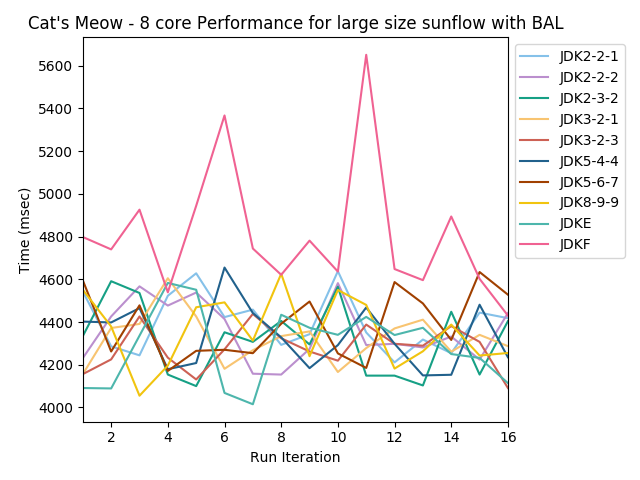
\includegraphics[width=0.8\linewidth, height=9cm]{HonoursReportTemplate_LaTeX/images/graphs/circling-8core-terminal/terminal-large-BAL-8core-sunflow.png}
       \caption{Performance time for \emph{sunflow} with Balanced}
\end{subfigure}
 \begin{subfigure}{1\textwidth}
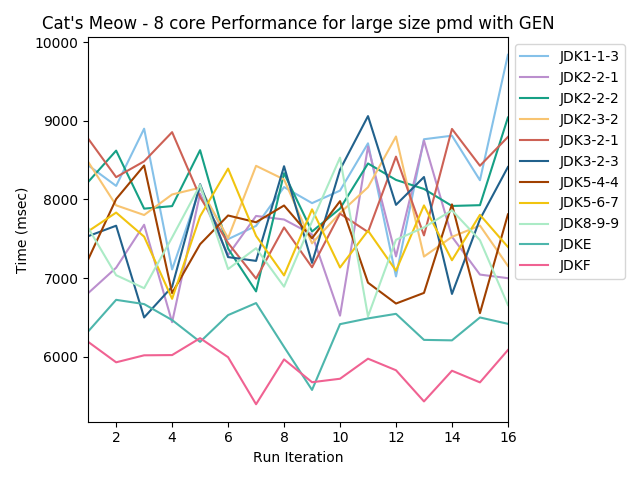
\includegraphics[width=0.8\linewidth, height=9cm]{HonoursReportTemplate_LaTeX/images/graphs/circling-8core-terminal/terminal-large-GEN-8core-pmd.png}
       \caption{Performance time for \emph{pmd} with GenCon}
\end{subfigure}

\caption{Performance for large sized benchmarks on 8-CPU machine with \emph{Circling} }
\end{figure}
\newpage
\begin{figure}[H]
\begin{subfigure}{1\textwidth}
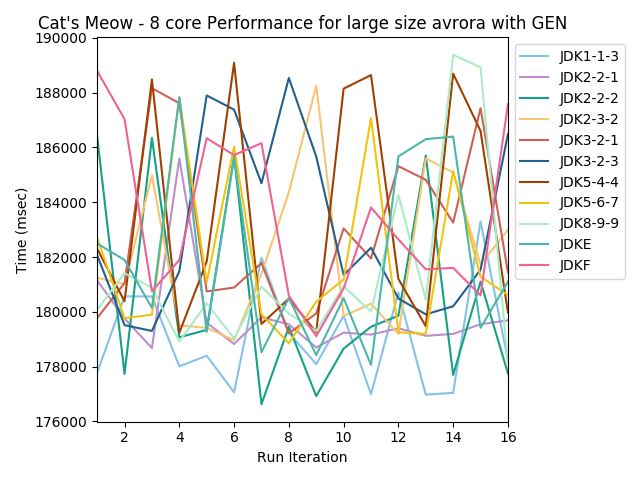
\includegraphics[width=0.8\linewidth, height=9cm]{HonoursReportTemplate_LaTeX/images/graphs/circling-8core-terminal/terminal-large-GEN-8core-avrora.png}
       \caption{Performance time for \emph{avrora} with GenCon}
\end{subfigure}

\begin{subfigure}{1\textwidth}
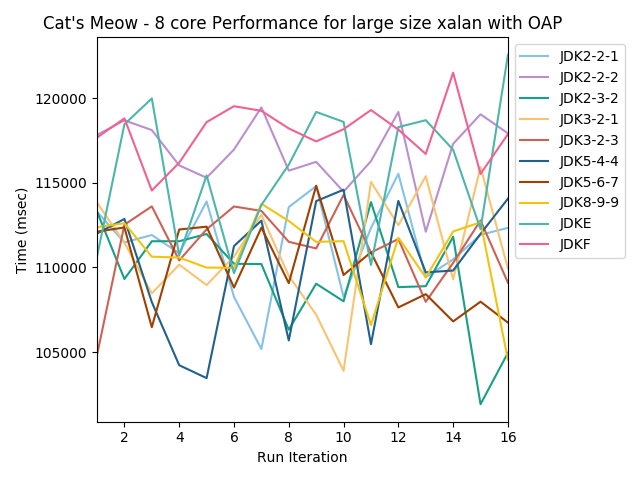
\includegraphics[width=0.8\linewidth, height=9cm]{HonoursReportTemplate_LaTeX/images/graphs/circling-8core-terminal/terminal-large-OAP-8core-xalan.png}
       \caption{Performance time for \emph{xalan} with OptAvgPause}
\end{subfigure}

    \caption{Performance for large sized benchmarks on 8-CPU machine with \emph{Circling} (1)}
    \label{fig:Circling-performance}
\end{figure}
\newpage
Based on the results from the testing conducted, it is clear that there
is a benefit to using the \emph{Circling} approach. The benefit is more
noticeable in longer-executing applications, particularly benchmarks
combined with policies that do not minimise pause times. However, the
PID controller appears to improve performance more so than GC
utilisation. Nevertheless, \emph{Circling} is an improvement over
\emph{CatNap}, naive threshold-based approach.

\subsection{Summary}
Using a PID controller provides performance benefits for applications
that do not have short execution times. There is some improvement in GC
utilisation with the PID controller implemented, but it is not
consistent. This research aims to manage GC utilisation and, thereby,
reduce the resource-intensiveness of GC. Hence, a different approach is
needed to manage GC utilisation better as the PID controller is not as
effective as expected. The next chapter discusses a \emph{Linear-Quadratic
Regulator} (LQR) and the impact of using an LQR on GC utilisation.

\newpage
\section{Cat's Meow}
The final development phase moves towards optimal control theory through
a Linear Quadratic Regulator (LQR). An LQR controls a system with minimal cost incurred to the system as described in
Chapter 2. It assumes that linear differential equations can describe
the system. Incorporating an LQR into the OpenJ9 JVM gives better
control over the GC utilisation as it makes decisions based on the model
of the system rather than merely making naive adjustments to variables.
This can be seen through most of the p-values falling below 0.05, and a
lower average when compared to the previous development phases for
OptAvgPause and OptThruPut.
\newline\newline
The phrase is named as \emph{Cat's Meow} as cats are able to adjust the tone of
their voice to achieve what they want. For example, a cat may sound
particularly sad in their meow to wake up an individual.

\subsection{Approach}
The approach for this phase is to develop an LQR that has the heap size, the
number of GC threads and the interval between local GC's as variables
that describe the state of the system. The \emph{lqr} control module provided
by Python is used to solve the Riccati equations, discussed in Chapter 2, and provide the matrix
for $K$ in $u = -Kx$. The conceptual background to an LQR is provided in
Chapter 2. The $K$ matrix defined by the \emph{lqr} control module forms an important part of the implementation of the LQR in the OpenJ9 JVM. 

\subsection{Implementation}
The LQR controller was implemented using a new struct: \verb|LQR|. 
This struct
contains each value of the $K$ matrix stored as a separate variable. The
use of individual variables is chosen in order to avoid the use of
array-like structures. In addition, an integral sum is used to ensure
values respond to the behaviour of the system, i.e. the adjustment of
values is dynamic and varies over time. This is important as the GC's
behaviour is not consistent throughout the runtime execution of a
program. The integral sum is set up similarly to how it was designed in
\emph{Circling} with a sliding window. The basic LQR controller without the
integral error sum is mathematically described below. Output weighting
is used with GC utilisation representing the desired output.
\newline\newline
\begin{math}
H( t) \ =\ heap\ size\ at\ time\ t\\
I( t) \ =\ interval\ between\ local\ GCs\ at\ time\ t\\
T( t) \ =\ number\ of\ GC\ threads\ at\ time\ t\\
uH( t) \ =\ used\ heap\ at\ time\ t\\
GP( t) \ =\ GC\ policy\ at\ time\ t\\
ar( t) \ =\ allocation\ rate\ of\ objects\ at\ time\ t\ or\ how\ the\ heap\ changes\ over\ time\ =\ \dot{uH( t)}\\
GC( t) \ =\ GC\ utilisation\ at\ time\ t
\end{math}
\newline\newline
The above functions are essential and comprise the initial model. These functions include the heap size, interval between local GCs and number of GC threads. The functions themselves are defined below.
\newline\newline
\begin{math}
H( t) \ =\ H( 0) \ +\ 65536k_{1}( t)\\
I( t) \ =\ I( 0) \ +\ k_{2}( t)\\
T( t) \ =\ T( 0) \ +\ k_{3}( t)\\
uH( t) \ =\ k_{4}( t)\\
ar( t) \ =\ \dot{k_{4}( t)} \ =\ \frac{k_{4}( t) \ -\ k_{4}( t\ -1)}{t\ -\ ( t\ -\ 1)}\\
GP( t) \ =k_{5}( t)\\
\\
where\ \ k_{1}( t) ,\ k_{2}( t) ,\ k_{3}( t) ,\ \ k_{4}( t) \ and\ k_{5}( t) \ are\ time-varying\ functions\ that\ are\ unknown\ and
\\ \\
65536\ is\ the\ default\ size\ of\ a\ region,\ a\ portion\ of\ the\ heap,\ in\ OpenJ9
\end{math}
\newline\newline
In the equations above, there are five unknown functions which are time variant. These functions are necessary as there are a lot of variables affecting GC and they cannot all be modelled. The functions above are used to define the model for the LQR as seen below.
\newline\newline
\begin{math}
x\ =\ \begin{bmatrix}
H( t)\\
uH( t)\\
ar( t)\\
GP( t)\\
I( t)\\
T( t)
\end{bmatrix}
\end{math}
\newline\newline
Therefore, this is the model of the system. This equation can be differentiated to give the following model where \begin{math} \dot{x} \end{math} represents the system differentiated over time. 
\newline\newline
\begin{math}
\dot{x} \ =\ \begin{bmatrix}
H'( t)\\
uH'( t)\\
ar'( t)\\
GP'( t)\\
I'( t)\\
T'( t)
\end{bmatrix}
\end{math}
\newline\newline
This becomes the following using the definitions of the functions above:
\newline\newline
\begin{math}
\dot{x} \ =\ \begin{bmatrix}
65536k_{1} '( t)\\
\ k_{2} '( t)\\
\ k_{3} '( t)
\end{bmatrix}
\end{math}
\newline\newline
In addition, \begin{math} \dot{x} \end{math} can be represented, based on the LQR theories, as the following:
\newline\newline
\begin{math}
\dot{x} \ =\ Ax\ +\ Bu
\end{math}
\newline\newline
where A is a matrix representing the system with no control, B is the effect of control and u is the input to the system. 
\newline\newline
For this system, the following assumptions are made:
\newline\newline
\begin{math}
It\ is\ assumed\ with\ no\ control\\
H'( t) \ =\ 0\\
I'( t) \ =\ 0\\
GP'( t) \ =\ 0\\
T'( t) \ =\ 0\\
\end{math}
\newline\newline
These assumptions are rational as it is normal that the GC variables do not change during runtime. For example, GC policy does not change during runtime. In addition, the number of threads and the interval between local GCs cannot currently change in the OpenJ9 JVM. The heap size can technically change during runtime; however, this model assumes that the application has been run numerous times so, the heap size is optimised to suit the application. 
\newline\newline
Despite the strength of this initial model, it is complex to form \begin{math} uH(t)\end{math} and \begin{math} ar(t) \end{math} as both these functions depend on previous state. Therefore, a simplified model is proposed instead with its corresponding differential:
\newline\newline
\begin{math}
x\ =\ \begin{bmatrix}
H( t)\\
I( t)\\
T( t)
\end{bmatrix}
\end{math}
\newline\newline
\begin{math}
\dot{x} \ =\ \begin{bmatrix}
H'( t)\\
I'( t)\\
T'( t)
\end{bmatrix}
\end{math}
\newline\newline
In addition, u, the input, is set to the following matrix:
\newline\newline
\begin{math}
u\ =\ \begin{bmatrix}
\alpha \\
\beta \\
\theta 
\end{bmatrix}
\end{math}
\newline\newline
Another component of the LQR is the following equation:
\newline\newline
\begin{math}
y\ =\ Cx\ +\ Du
\end{math}
\newline\newline
Based on this system, y is equal to: 
\newline\newline
\begin{math}
y\ =\ GC( t) \ =\ K_{1} H( t) \ +\ K_{2} I( t) \ +\ K_{3} T( t)\\
\\
where\ K_{1} ,\ K_{2} \ and\ K_{3} \ are\ variables
\end{math}
\newline\newline
Therefore, moving back to:
\newline\newline
\begin{math}
\dot{x} \ =\ Ax\ +\ Bu
\end{math}
\newline\newline
It is possible to make this assumption, as described above, that \begin{math} A = 0 \end{math}. Therefore, the equation becomes 
\begin{math}
\dot{x} \ =\ Bu
\end{math}
\newline\newline
which becomes
\newline\newline
\begin{math}
\dot{x} \ =\ B\ \begin{bmatrix}
\alpha \\
\beta \\
\theta 
\end{bmatrix}
\end{math}
\newline\newline
and, therefore, this
\newline\newline
\begin{math}
\begin{bmatrix}
65536k_{1} '( t)\\
\ k_{2} '( t)\\
\ k_{3} '( t)
\end{bmatrix} =\ B\ \begin{bmatrix}
\alpha \\
\beta \\
\theta 
\end{bmatrix}
\end{math}
\newline\newline
and B becomes, through matrix multiplication:
\newline\newline
\begin{math}
B\ =\ \begin{bmatrix}
65536 & 0 & 0\\
0 & 1 & 0\\
0 & 0 & 1
\end{bmatrix}\\
\\
assuming\ that\ \alpha \ \rightarrow \ k_{1} '( t)\\
\beta \ \rightarrow \ k_{2} '( t)\\
\theta \ \rightarrow \ \ k_{3} '( t)
\end{math}
\newline\newline 
The system is controllable and observable as the rank of B and \begin{math} \dot{x} \end{math} is 3. 
\newline\newline
The use of Python's \emph{lqr} control modules requires the determining of Q and R from the Riccati equations provided in Chapter 2. Output weighting is used to determine Q as the output, GC utilisation should be minimised. In addition, R is set to three times the identity matrix to simplify the model and ensure the final values from the \emph{lqr} module are appropriate for the model. 
\newline\newline
Therefore, Q and R are as follows:
\newline\newline
\begin{math}
Q\ =\ H^{T} H\ \\ \\
where\ y\ =\ Hx\\
\\
y\ =\ Hx\\
K_{1} H( t) \ +\ K_{2} I( t) \ +\ K_{3} T( t) \ =\ H\begin{bmatrix}
H( t)\\
I( t)\\
T( t)
\end{bmatrix}\\
\\
\therefore H\ =\ \begin{bmatrix}
K_{1} & K_{2} & K_{3}
\end{bmatrix}\\
\\
Q\ =\ \begin{bmatrix}
K^{2}_{1} & K_{1} K_{2} & K_{1} K_{3}\\
K_{2} K_{1} & K^{2}_{2} & K_{2} K_{3}\\
K_{3} K_{1} & K_{3} K_{2} & K^{2}_{3}
\end{bmatrix}\\
\\
R\ =\ I\ =\ \begin{bmatrix}
1 & 0 & 0\\
0 & 1 & 0\\
0 & 0 & 1
\end{bmatrix}
\end{math}
\newline\newline
It is the \begin{math}  K_{1}, K_{2}, K_{3} \end{math} that determine the different values of the LQR controller as they feed into the \begin{math}K\end{math} matrix, which sets the input,\begin{math} u\end{math}. Hence, it is these different \begin{math}K \end{math}values that correspond to the names of the different JVMs created in this development phase. 
\newline\newline
In terms of code, the following steps were followed in the
\emph{ParallelDispatcher} code to integrate the \emph{LQR} controller within the
original GC logic:

\begin{enumerate}
\def\labelenumi{\arabic{enumi}.}
\item
 
  Set  \begin{math}  K_{1}, K_{2}, K_{3} \end{math}  values.
\item

  Set the initial number of threads, heap and interval.

\item
 
  Calculate integral error.
 
\item

  Calculate new heap size.
 
\item
  
  Calculate new interval.
  
\item
 
  Calculate new thread count.
 
\item

  Confirm new changes are valid.

\end{enumerate}
Similar to the limits put on the variables in \emph{CatNap}, the heap size is
limited to the maximum and minimum values set by the JVM initially. In addition,
the maximum number of GC threads are limited to the number of CPU cores,
and the maximum interval of local GCs allowed is 4000 msec.

\subsection{Testing}
The same approach used for \emph{Circling} and \emph{CatNap} was applied to
ensure comparability. Hence, 4-CPU and 8-CPU Linux Virtual Machines
are used along with chosen DaCapo benchmarks. This allows comparability
between the different development phases.
\newline\newline
There are nine different versions of the \emph{Cat's Meow} mode. These versions
represent different combinations of \begin{math}  K_{1}, K_{2}, K_{3} \end{math} values. The choice
of values is determined by the \emph{lqr} control module in Python to ensure
that the values create eigenvalues in the left-hand plane. Having
eigenvalues in the left-hand plane ensures the system is stable. The
configuration of values are calculated using the \emph{lqr} control module in Python. These
values are chosen as the eigenvalues for all of these values were in the
left-hand plane, meaning the system is stable. The stability of a system
is critical, noted in Chapter 2, as it ensures that the system does
not begin oscillating.
\newline\newline
The different combinations are listed below in the table, along with the
overall relationship and the individual values. In addition to the JVMs
listed, there are also two other JVMs; JDKF and JDKE. JDKF is the
original JVM without any modifications beyond the ability to log GC
utilisation and the time the application has been running. In a similar
vein, JDKE is the modified JVM without enabling \emph{Cat's Meow} mode while
still logging the GC utilisation and the time the application has been
running.
\newline\newline
\begin{table}[H]
\begin{tabular}[]{|c|c|c|c|}
\hline
Name & Value of K1 & Value of K2 & Value of K3\tabularnewline
\hline
JDK1-1-3 & 1 & 1 & 3\tabularnewline \hline

JDK2-2-1 & 2 & 2 & 1\tabularnewline \hline

JDK2-2-2 & 2 & 2 & 2\tabularnewline \hline

JDK2-3-2 & 2 & 3 & 2\tabularnewline \hline

JDK3-2-1 & 3 & 2 & 1\tabularnewline \hline

JDK3-2-3 & 3 & 2 & 3\tabularnewline \hline

JDK5-4-4 & 5 & 4 & 4\tabularnewline \hline

JDK5-6-7 & 5 & 6 & 7\tabularnewline \hline

JDK8-9-9 & 8 & 9 & 9\tabularnewline \hline
\end{tabular}
\caption{Modified JVM's implementing the described LQR controller for \emph{Cat's
Meow}}
\end{table}
The above-described combinations aim to reflect the total number of
possible relationships for different $K$ values. Using different JVMs
identifies the combination of $K$ values most appropriate for reducing GC
utilisation.

\subsection{Results}
Implementing an LQR controller allows for greater control over GC
utilisation as reflected by the results of \emph{Cat's Meow}. A similar
discussion to the earlier development phases is provided for the
results from \emph{Cat's Meow} below.
\subsubsection{P-values}
The p-values show that there is a statistically significant difference
between the original JVM of JDKF and the modified JVMs for most of the
benchmarks with OptAvgPause and OptThruPut in terms of GC utilisation. In contrast, \emph{pmd} for GenCon
does not have statistically significant values for all of the modified
JVMs. It is a similar result for the p-values for \emph{sunflow} with Balanced.
The consequences of these p-values mean that the null hypothesis can be
rejected for the modified JVMs for most of the benchmarks run with
OptAvgPause or OptThruPut. The null hypothesis cannot be rejected for
pmd with GenCon. The p-values are provided below. Statistically significant values are bolded in the tables. 
\newline\newline
The full summary statistics are available through a shared link provided
in Appendix A. These statistics include standard deviation, root mean
squared error and mean.

\subsubsection{Mean}

The findings from the p-values table above are reiterated by the mean GC
utilisation graphs provided on the next page. For the benchmarks run
with OptAvgPause, there is a significant difference between the mean GC
utilisation of the modified JVMs and the original JVM, JDKF. The
difference is more noticeable for \emph{jython} than for the other benchmarks.
It was mentioned in Chapter 3 that \emph{jython} creates a large number of
objects on the heap. Therefore, the results from this phase indicate
that the LQR controllers are better able to manage applications with
many objects.
\newline\newline
In contrast to OptAvgPause is GenCon, where the mean GC utilisation
tends higher than JDKF. The exception is \emph{xalan}, which shows lower GC
utilisation than JDKF. Again, \emph{xalan} has a high allocation rate of
objects to the heap meaning the conclusion made for \emph{jython} applies to \emph{xalan}. 
\newline\newline
Generally, the standard error for the mean GC utilisation is relatively small. An exception is JDK-1-1-3 with \emph{sunflow} and a Balanced GC policy. This variance reflects the variability of the GC with JDK1-1-3 combined with a Balanced GC policy. With this JVM and policy, GC utilisation tended to differ across each test run thus showing that the model with its  \begin{math} K\end{math} values is not as appropriate with the combination of policies and benchmark. 
\newline\newline
It is also noticeable that OptAvgPause and OptThruPut perform better than Balanced and GenCon. This better performance indicates that these policies align more with the LQR model created. In addition, it implies that the impact of generational garbage collection needs to be considered in an LQR model as both Balanced and GenCon have some form of generational garbage collection. 

\subsubsection{GC Utilisation}
The spread of GC utilisation over time again echoes the p-value
findings. JDKF and JDKE, the modified JVM without the modifications
enabled, tends to have higher GC utilisation than the modified
JVMs for OptAvgPause and OptThruPut. The two unmodified JVMs, JDKF and JDKE, have a
different trend tending towards an inverse parabolic curve. In contrast,
the modified JVMs tend towards a very shallow parabolic curve. An
example of \emph{sunflow} with OptThruPut is provided on the next page. This
variance between JDKF or JDKE and the modified JVMs is not observable when using the GenCon or Balanced policies.
\newline\newline
Some of the GC utilisation readings appear to tend towards 0\% on the graphs on the next page. These low GC utilisation readings reflect the variable nature of GC utilisation meaning it can both spike up and down. Generally, GC utilisation will approximate to 0\% at the beginning of runtime. After that, GC utilisation will only tend closer to 0\% if the time spent in GC is minimal comparatively. Minimal time spent in the GC is more likely to occur with GC policies that avoid or minimise GC pauses, such as OptAvgPause. In addition, OptThruPut may see similar behaviour if global GCs are less frequent.   

\subsection{Summary}
Using an LQR controller provides better management of GC utilisation in
particular scenarios where there is a high allocation rate or objects in
the heap size and using OptAvgPause and OptThruPut policies. An LQR
controller is less effective when combined with GenCon or Balanced
policies. The effectiveness of these LQR controllers indicates that the
model used to formulate the LQR is reasonably accurate. The next chapter
further evaluates this model as well as the PID controller by testing
the JVMs in a multitenant environment.

\newpage
\section{Many Cats On A Bed}
This research aims to reduce GC-related spikes that cause
performance interference in multitenant scenarios. The prior development
phases have focused on the performance of \emph{A Cat on a Bed} for an
individual JVM. This section instead focuses on the multitenant
scenario, research question 2, and how \emph{A Cat on a Bed} functions with
other JVMs. Addressing this research question requires forming a game
theory model and testing in multitenant scenarios with Kubernetes. The
approach is separated into two areas: theoretical, relating to game
theory, and practical, applying Kubernetes.
\subsection{Theoretical approach (Game theory)}
For the game theory approach, the discussion provided in Section 2
provides most of the methodology for applying game theory to multitenant
scenarios for this research. The model is simplified by limiting
multitenant scenarios to two co-located tenants on a VM.
\newline\newline
The players for the game theory model are the different tenants
co-located on a specific VM. Players are rational and are trying to
maximise their utility. Utility represents, for this scenario,
increasing their resources to finish the execution of their
applications. The players can take the following actions, which are
scheduled by the controller:
\begin{itemize}
\item
  Decrease the number of used CPU cores
\item
 Increase the number of used CPU cores
\item
  Do nothing
\end{itemize}
In terms of the game, each game is simultaneous as all of the moves
will technically be made at the same time. There is imperfect
information as the players do not know what other players are doing.
Furthermore, a player does not know the predicted resource utilisation
of another or themselves. Players are non-cooperating as there is no
fixed agreement between them.
\newline\newline
The game was limited to two players to simplify the model. However,
it could be extended by adding more matrices for payoffs. The payoffs are
determined arbitrarily based on the assumption that everyone is punished
if the entire VM overuses its resource allocation. This is aligned with
the fact that if a pod, seen as a VM, requests too many resources, it
may be evicted. There is also an assumption that payoffs are determined
by the likelihood of breaking resource allocation thresholds.
\newline\newline
There is the assumption that the players are not related, i.e. they
are not dependent on each other. An example of related players is those
part of microservice applications. These applications require different
components to communicate with each other, such as passing data between
the components. The rationale behind excluding scenarios where there are
related players is that it would be expected that the players would
naturally coordinate their actions and resource usage.
\newline\newline
Therefore, this research focuses on unrelated players in multitenant
scenarios. In terms of the development of the game theory model,
arbitrary payoffs are assigned to the different decisions/actions of the
players. These payoffs can be formalised and sourced directly from the
Service Level Agreements (SLAs) from a cloud provider. The following
paragraph shows the logic applied to calculate the payoffs. In the figure,
there is reference made to `increases` and `decreases`, this should be
interpreted as `increases resource usage` and `decreases resource
usage`.
\newline\newline
The  logic applied to calculate the payoffs for the game
theory model includes:

\begin{itemize}
\item
If Player 1 increases and Player 2 decreases
  \begin{itemize}
  \item
    The chance of breaking resource allocation threshold is
    unchanged.
  \item
    Player 1 receives more benefit as it can use the resources
    technically freed by Player 2, so payoff is 10.
  \item
  Player 2 receives no benefit and instead incurs a cost as it is
    letting Player 1 use resources without improving the chance of
    breaking resource allocation threshold. Payoff is -5.
  \end{itemize}
\item
 If Player 1 decreases and Player 2 decreases

  \begin{itemize}
  \item
   The chance of breaking resource allocation threshold decreases.
  \item
    Player 1 receives benefit, so payoff is 5.
  \item
   Player 2 receives benefit, so payoff is 5.
  \end{itemize}
\item
 If Player 1 increases and Player 2 does nothing
  \begin{itemize}
  \item
    The chance of breaking resource allocation threshold is
    heightened as Player 1 has increased its resource utilisation.
  \item
    Player 1 increases its resource usage unnecessarily and is
    directly responsible for the increase in the chance of breaking
    resource allocation threshold as well. Payoff is -5.
  \item
   Player 2 has done nothing but is also indirectly responsible for
    the increase in the chance of breaking resource allocation threshold
    as well. Payoff is -2.5.
    \end{itemize}
  \item
  If Player 1 decreases and Player 2 stays the same.
    \begin{itemize}
    \item
    The chance of breaking the resource allocation threshold
      decreases.
    \item
     Player 1 has sacrificed some of its resources, costing its
      ability to execute its applications. Payoff -2.5.
    \item
    Player 2 has done nothing without sacrificing any ability to
      execute applications. Payoff 2.5.
    \end{itemize}
  \item
  If Player 1 does nothing and Player 2 does nothing
    \begin{itemize}
    \item
      No change in the chance of breaking the resource allocation
      threshold.
    \item
     Player 1 does nothing and does not reduce the chance of
      breaking the resource allocation threshold. Payoff -2.5.
    \item
      Player 2 does nothing and does not reduce the chance of
      breaking the resource allocation threshold. Payoff -2.5.
    \end{itemize}
  \item
    If Player 1 increases and Player 2 increases.
    \begin{itemize}
    \item
     The chance of breaking the resource allocation threshold is
      significantly worsened.
    \item
      Player 1 has directly influenced and worsened the chance of
      breaking the resource allocation threshold. Payoff -5.
    \item
      Player 2 has directly influenced and worsened the chance of
      breaking the resource allocation threshold. Payoff -5.
    \end{itemize}
\end{itemize}
The above logic can also be expressed in a matrix.
\begin{table}[H]
\centering
\begin{adjustbox}{width=\textwidth}
\begin{tabular}{|c|c|c|c|c|}
\hline
&     & \multicolumn{3}{l|}{Player 2} \\
\hline
      &  & Increase number of CPU cores & Decrease number of CPU cores & Do nothing \\ \hline
\multirow{3}{*}{Player 1} & Increase number of CPU cores & -5,-5                        & 10,-5                        & -5, -2.5   \\ \hline
                          & Decrease number of CPU cores & -5, 10                       & 5, 5                         & -2.5, 2.5  \\ \hline
    & Do nothing                   & -2.5, 5                      & 2.5, -2.5                    & -2.5, -2.5  \\ \hline
\end{tabular}
\end{adjustbox}
\end{table}
Currently, each player does not consider and is not aware of the
other player. A player can assume a worst-case scenario where the other
player will choose to increase their number of CPU cores as it will see
a maximum payoff of 10. Therefore, the best decision for the other
player, only considering themselves, will be to do nothing. If the
player considers the whole game, the best decision is to decrease their
number of CPU cores. In contrast, if a player assumes that the other
player will choose to do nothing, then the player should also do nothing
to achieve the best payoff. This assumption, again, only considers the
players' individual gains. It should be
noted that the most gain is received for the whole game is 10 if both
players decrease their number of CPU cores.
\newline\newline
From Chapter 2, Nash's equilibrium exists where both players are not
motivated to change their decisions. In theory, Nash's equilibrium for
the above payoff matrix is for both players to do nothing assuming they
do not know what the other player will do. This is because this provides
a player with the best payoff irrespective of what the other player
does. Nevertheless, a better decision for both players is to reduce
their resource usage; however, this is unlikely in real multitenant
scenarios. Nash's equilibrium of the players doing nothing provides a
rationale for why users of clouds do not reduce their resource usage.

\subsection{Practical approach (Kubernetes)}
In addition to the theoretical approach described above, \emph{A Cat On A
Bed} is implemented on Kubernetes. Using Kubernetes allows for the
simulation of multitenant clouds. Applying \emph{A Cat On A Bed} to a realistic
multitenant scenario is essential in evaluating its' effectiveness in
managing GC utilisation when there is more than one application. This practical approach
addresses research question 1.

\subsubsection{Approach}

The goal of this part is to evaluate \emph{A Cat On A Bed's} performance
in multitenant scenarios. In Kubernetes, multitenant scenarios with shared resources occur
within a Pod with multiple containers; therefore, the testing focuses on a single Pod with either
one or two containers. Evaluating the performance of the JVMs is
accomplished through measuring the CPU utilisation, memory utilisation,
GC utilisation and performance time. In addition, the performance of a
JVM is significantly reduced if the Pod is evicted.
\subsubsection{Testing}

A selection of the JVMs from previous development phases was tested
in this phase. The chosen JVMs are listed below:
\begin{itemize}
\item
  JDKF
\item
  JDK0.5-0.5-1 (PID controller)
\item
  JDK1-1-3 (LQR controller)
\item
 JDK2-2-2 (LQR controller)

\item
  JDK2-3-2 (LQR controller)

\end{itemize}
The selection of JVMs is based on the results from the previous
phases. Generally, these selected JVMs performed well. Multiple JVMs
from Cat's Meow (the \emph{Linear-Quadratic Regulator} Controller phase) are
chosen as it was difficult to differentiate the better performer across
the different benchmarks or policies. JDKF, the original JVM, is tested
again to provide a benchmark of how the JVM typically performs on
Kubernetes.
\newline\newline
Based on the results from \emph{Circling} and \emph{Cat's Meow}, the testing suite
changed from individual benchmarks to running the five benchmarks in one
test run. This change in testing aims to address two considerations:
firstly, \emph{Circling} is not well suited to short-run applications, and
secondly, multitenant clouds generally have applications that tend to
longer execution time \cite{shen2011cloudscale}. Both of these
considerations meant that it was appropriate to have longer run tests.
The tests are, again, run with the four different GC policies and
repeated 16 times.
\newline\newline
In addition, as Kubernetes is a different environment to the earlier
testing environment for \emph{CatNap, Circling, and Cat's Meow}, the
testing for this phase is structured differently. It is
important to establish a baseline for all of the JVMs on Kubernetes to
understand their typical behaviour. This is achieved through testing a
single container in a Pod for each JVM. The multitenant aspect is tested
by having two containers in a Pod for each JVM. The containers are the
same JVM. Details of the setup files used for Kubernetes are provided in
Appendix A in a Github link. Future work could combine different JVMs to
identify if there is a change in performance and GC utilisation
management.
\newline\newline
The \emph{minikube} environment is used for running the tests, and it is
configured with 16-CPU cores and 16384 MB of memory. No attempt is made
to set the number of CPUs that the different or single container uses.
The rationale behind using \emph{minikube} is that it is suitable for the small
scope of testing and is compatible with appropriate add-ons, i.e.
\emph{metrics-server}. The add-on mentioned, \emph{metrics-server}, is required to
collect memory and CPU utilisation statistics.
\subsubsection{Results}
The focus of this phase is on multitenant scenarios; therefore,
evaluation of the different JVMs focuses on different vital statistics.
These statistics include GC utilisation, performance time, memory
utilisation and CPU utilisation. The statistics are separated into the
single container in a Pod and two containers in a Pod. Generally, the
findings reiterate the findings from earlier development phases; LQR
controllers are better at managing GC utilisation, whereas PID
controllers reduce execution time. In addition, PID controllers have
lower CPU utilisation linking to better performance. PID
controllers also have higher memory utilisation that reflects their
lowered ability to manage GC utilisation.
\newline\newline
\textbf{Single container in Pod}
\newline\newline
In terms of GC utilisation for a single container, there is a clear
trend that the LQR controllers have lower GC utilisation for GC policies
other than GenCon. JDK0.5-0.5-1, a PID controller, has less frequent GCs
than JDKF, the original JVM, and the LQR JVMs. The lower GC utilisation
for the JVMs with LQR controllers is more apparent with OptThruPut and
OptAvgPause. In contrast, JDK0.5-0.5-1 has similar GC utilisation to the
other LQR JVMs for GenCon and Balanced. Nevertheless, JDKF generally has
higher GC utilisation. These results can be observed from the next page of
graphs.
For CPU utilisation and a single JVM, there is generally lower CPU
utilisation for JDK0.5-0.5-1 (PID controller) compared to the other JVMs. This lower CPU utilisation reflects the
lowered performance time as well. In terms of the three LQR controllers,
there is little difference between their CPU utilisation and JDKF's, the
original JVM, irrespective of GC policy. There are similar results for
memory utilisation. These results can be seen in the graphs provided on
the next page. Not all of the graphs have the same scale because some of
them, particularly JDK0.5-0.5-1, have lower utilisation. Graphing on the
same scale makes it difficult to observe any trends within the separate
JVMs.

Similar to the findings from the earlier phases, JDK0.5-0.5-1 takes
a shorter time to execute the test benchmarks. This shorter time is more
apparent with OptThruPut and OptAvgPause. In addition, JDK1-1-3,
JDK8-9-9, JDK2-2-2 and JDK2-3-2 have worse performance than JDKF
irrespective of GC policy. The graphs relating to performance time are
provided on the next page.
The results from two containers in a Pod are similar to the results
from one container in a Pod; however, there are some slight differences
relating to the prioritisation of different containers.
\newline\newline 
The results for GC utilisation show that, irrespective of which
container is prioritised, GC utilisation is similar to the GC
utilisation for a single container in a Pod. In addition, GC utilisation
for each container is usually around the same value. Again, the LQR
controllers perform better in terms of GC utilisation management. The better management of GC utilisation by the LQR controllers
is reflected in the graphs below and on the next page. GC utilisation is also
lower with OptThruPut and OptAvgPause policy compared to Balanced and
GenCon. These findings for GC utilisation reiterate the findings from
earlier phases.
CPU utilisation and memory utilisation tend to have similar
patterns. Overall, having two containers in a Pod does not affect the
CPU utilisation and memory utilisation compared to having one container
in a Pod; therefore, similar results for a single container in a pod
apply to two containers in a pod. However, this perspective of the
results occur when an overall view is taken, i.e. the two containers'
memory and CPU utilisation are taken together. Separately, it is clear
that one of the containers will usually have lower CPU utilisation and
memory utilisation even compared to the results earlier for a single
container in a pod. Another difference is that JDK0.5-0.5-1 does not
perform as well with two containers in a pod. For example, with two
containers, the memory utilisation spikes to 4000MiB for OptThruPut
policy compared to JDKF's, the original JVM, highest spike of
400\% for OptThruPut policy. This spike for JDK0.5-0.5-1 is unexpected,
considering the better performance of the JVM for one container in a
pod. An excerpt of the graphs is provided below.
Graphing the performance times of the different JVMs reiterates the
findings from a single container in a Pod; JDK0.5-0.5-1 has better
performance and the LQR JVMs have the worst performance. In addition, it
appears that there is an inverse relationship between the performance
time of the two containers in a Pod, i.e. one container has lower
performance time, and the other container then has a higher performance
time. Having this type of relationship indicates the impact of
multitenant scenarios. Furthermore, there is a lower difference between
the two containers' performance for the modified JVM's shown by a
smaller distance between the two containers for the modified JVMs on the
graphs. These graphs are provided on the next page.
\subsection{Summary}

Multitenant scenarios are a crucial facet of this research and are
addressed through a theoretical approach, game theory, and a practical
approach focusing on Kubernetes. The theoretical approach, game theory,
shows that Nash's equilibrium exists where both players do nothing;
however, a better alternative is for the players to decrease their
resource usage. In terms of the practical approach, the results
reiterate the findings from the earlier phases relating to performance
time and GC utilisation. These findings show that an LQR controller in
the JVM is better for controlling GC utilisation but does not have a
positive impact on performance time. In contrast, a PID controller in the
JVM is better in reducing performance time but is not effective in
managing GC utilisation.



\newpage
\section{Conclusion}

In approaching this research, there were two research questions:
\begin{itemize}
\item

  Will an elastic GC mode that varies the heap size, number of threads
  and interval between standard GC's see a reduction in GC utilisation
  and hence overall CPU utilisation?
  
\item

  Is it possible to formulate Nash's equilibrium for co-located tenants
  using the elastic GC mode to reduce performance interference overall?
  
\end{itemize}
Based on the three development phases, it is clear that it is possible
to manage and reduce GC utilisation both in single VM and multitenant
scenarios; thus, addressing the first research question. The development
phases also highlight that reducing GC utilisation can harm performance
time of applications. Generally, the naive threshold-based approach,
CatNap, was ineffective in managing GC utilisation. The other two
phases, Cat's Meow and Circling, were more effective than CatNap showing
that control-theory motivated approaches are appropriate for this
research problem. Furthermore, an LQR is better for GC utilisation
control but only with particular GC policies, OptAvgPause and
OptThruPut, and applications with high allocation rates or large number of
objects in a heap. The positive impact of the Cat's Meow JVMs, which
implemented an LQR controller, indicates that concurrent GC policies,
such as OptAvgPause and OptThruPut, work well with LQR controllers. The
PID controllers implemented in Circling showed better performance time,
meaning that the gain in other areas outweighs the cost of adding the
PID controller logic. However, Circling JVMs did not see a significantly
noticeable improvement in GC utilisation, meaning the benefits from the
PID controller must result in time gains in other areas in a JVM.
\newline\newline
The multitenant testing reiterated the findings from the single VM. It
further proved that the benefits of the different JVMs from Circling and
Cat's Meow are observable in multitenant scenarios. In addition, CPU
utilisation reduces for Circling JVMs, but it is less noticeable for
Cat's Meow JVMs.
\newline\newline
A game theory model was formed to address the second research question.
The model showed that Nash's equilibrium is met if both tenants do
nothing. However, this is not an ideal solution and indicates that there
needs to be an adjustment to how tenants view gains in cloud computing
to ensure tenants are motivated to reduce their resource usage.
\newline\newline
Therefore, based on the findings from this research, the initial
hypotheses were correct. These hypotheses were that it would be possible
to reduce GC utilisation and formulate Nash's equilibrium. However, the
reduction of GC utilisation primarily occurs with an LQR controller but
is dependent on the benchmarks and GC policies.

\subsection{Contribution}

This research makes the following contributions:

\begin{itemize}
\item
  A PID controller-driven elastic GC mode implemented on OpenJ9 that effectively reduces execution time of applications
\item
  An LQR controller-driven elastic GC mode implemented on OpenJ9 that better manages GC utilisation
\item
  A game-theoretic model for two co-located tenants on a multitenant
  environment
\end{itemize}

\subsection{Limitations}
One limitation of this research is the sole use of DaCapo benchmarks
\cite{blackburn2006dacapo}. Additional benchmark suites could
have been used to substantiate the results. Other benchmarks that were
considered include Renaissance \cite{prokopec2019renaissance} and
CloudSim \cite{calheiros2011virtual}. These benchmarks were not
used in this research due to the scope and timing of the research.
\newline\newline
Another limitation is the simplification of the GC model applied in
Cat's Meow. The model used simplifies the GC to being described by the
three chosen variables: heap size, number of GC threads and the interval
between local GCs. This is an over-simplification of the entire GC model
but was needed to provide proof-of-concept that LQR is an appropriate
approach for the research problem. Future work could focus on creating a
realistic GC model for the Eclipse OpenJ9 JVM.

\subsection{Future Work}
Potential future work from this research has already been referenced in
earlier parts of this dissertation. Generally, most future work focuses
on the further development of the existing models, i.e. LQR and PID. In
addition, a broader scope of testing suites could be used to evaluate
the different development phases better. A final area for future work is
evaluating the modes on realistic multitenant clouds to identify the
implications of adjusting GC resource utilisation.




\newpage
\bibliographystyle{apacite}
\bibliography{biblio}
\newpage 
\appendix
\section{Appendices}
\subsection{Github Repositories and Summary Statistics}
\input{HonoursReportTemplate_LaTeX/githubrepo.tex}
\newpage
\subsection{Interim Report}
\input{HonoursReportTemplate_LaTeX/interim.tex}
\end{document}
